\documentclass[pdf]{beamer}
\mode<presentation>{\usetheme{Singapore}}
\beamertemplatenavigationsymbolsempty
\title{Leader Election in Arbitrary, Asynchronous Networks}
\author{Michele Castrovilli, Mattia Cerrato, Pasha Ostadi}
\usepackage{default}
\usepackage{graphicx}
\graphicspath{{./img/}}
\usepackage{tcolorbox}
\usepackage{tikz}
\usetikzlibrary{arrows}

\begin{document}
\Large
\begin{frame}
    \maketitle
\end{frame}

\normalsize
\begin{frame}{Overview}
    \begin{itemize}
        \item Leader Election: a short review
        \item Floodmax in the asynchronous model
        \item Why use searching/tree building algorithms?
        \item Spanning trees
        \item Breadth-first search
        \item Bellman-Ford algorithm 
    \end{itemize}
\end{frame}

\section{Leader Election}
\begin{frame}{Leader Election}
    Finding a leader node is an important problem in distributed systems.
    
    \vspace{12pt}
    \textbf{Motivation}: A leader node is a node in the network with additional responsibilities.
    \begin{itemize}
        \item Communication
        \item Coordinating data processing
        \item Allocating resources
        \item Token re-generation
   \end{itemize} 
\end{frame}

\begin{frame}{Leader Election}
    \textbf{Problem}: Breaking the Symmetry 
    
    \vspace{12pt}
    Each process has the same code. How do we elect a single leader?
    
    \vspace{12pt}
    Common techniques include the usage of randomness and/or unique process identifiers (\textbf{UIDs}).
\end{frame}

\section{Floodmax}

\begin{frame}{Synchronous Floodmax}
    \textbf{Assumptions}:
    \begin{itemize}
        \item The system is synchronous;
        \item Processes have unique identifiers (UIDs);
        \item The diameter, \textbf{diam}, is known to each process.
    \end{itemize}
    
    \vspace{12pt}
    \textbf{Result}:
    Exactly one process should elect itself the leader.
\end{frame}

\begin{frame}{Synchronous Floodmax}
    \vspace{12pt}
    Each node knows the diameter \emph{diam} of the network, and has an unique identifier, UID. \\
    For every round from 0 to \emph{diam}:
    \begin{enumerate}
        \item Send the maximum ID you found so far
        \item Receive another ID, $ID_{2}$. If $ID_{2} >$ UID, \\
         UID $\leftarrow$ $ID_{2}$ 
    \end{enumerate}
    After \emph{diam} rounds, every process will have the maximum UID of the network.
    If that UID corresponds to its own, the node will elect itself as the leader.
\end{frame}

\begin{frame}{Asynchronous Floodmax}{FloodMax}
    The FloodMax algorithm can be extended to the asynchronous network, by simulating
    the rounds.\\
    So, each process:
    \vspace{12pt}
    \begin{enumerate}
        \item Sends messages tagged with the round number; \\
        \item When it has received the round $r$ messages from its neighbors, moves on to the next round; \\
        \item Terminates after $diam$ rounds have been simulated. \\
    \end{enumerate}
\end{frame}

\begin{frame}{Asynchronous Floodmax}{Simulation (1 of 3)}
\begin{columns}
\begin{column}{.4\textwidth}
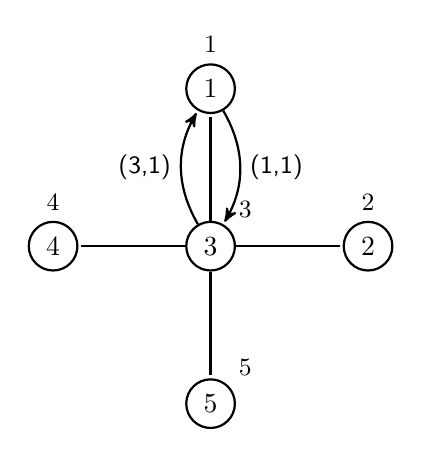
\begin{tikzpicture}[>=stealth',shorten >=1pt,auto,node distance=2cm,
                    thick,main node/.style={circle,draw,font=\normalsize}]
  \node[main node,label=above:{\small 1}] (1) {1};
  \node[main node,label=45:{\small 3}] (3) [below of=1] {3};
  \node[main node,label=above:{\small 2}] (2) [right of=3] {2};
  \node[main node,label=above:{\small 4}] (4) [left  of=3] {4};
  \node[main node,label=45:{\small 5}] (5) [below of=3] {5};
  \path[every node/.style={font=\sffamily\small}] 
    (1) edge [->,bend left] node [right] {(1,1)} (3)
    (3) edge [->,bend left] node [left] {(3,1)} (1)
    (3) edge node {} (1)
    (3) edge node {} (2)
    (3) edge node {} (4)
    (3) edge node {} (5)
    ;
\end{tikzpicture}
\end{column}
\vrule{}
\hspace*{10pt}
\begin{column}{.4\textwidth}
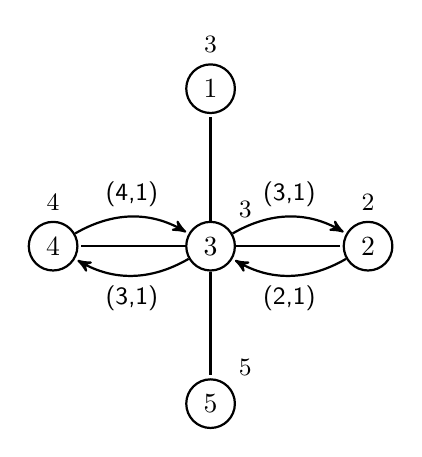
\begin{tikzpicture}[>=stealth',shorten >=1pt,auto,node distance=2cm,
                    thick,main node/.style={circle,draw,font=\normalsize}]
  \node[main node,label=above:{\small 3}] (1) {1};
  \node[main node,label=45:{\small 3}] (3) [below of=1] {3};
  \node[main node,label=above:{\small 2}] (2) [right of=3] {2};
  \node[main node,label=above:{\small 4}] (4) [left  of=3] {4};
  \node[main node,label=45:{\small 5}] (5) [below of=3] {5};
  \path[every node/.style={font=\sffamily\small}] 
    (2) edge [->,bend left] node [below] {(2,1)} (3)
    (3) edge [->,bend left] node [above] {(3,1)} (2)
    (4) edge [->,bend left] node [above] {(4,1)} (3)
    (3) edge [->,bend left] node [below] {(3,1)} (4)
    (3) edge node {} (1)
    (3) edge node {} (2)
    (3) edge node {} (4)
    (3) edge node {} (5)
    ;
\end{tikzpicture}
\end{column}
\end{columns}
\end{frame}

\begin{frame}{Asynchronous Floodmax}{Simulation (2 of 3)}
\begin{columns}
\begin{column}{.4\textwidth}
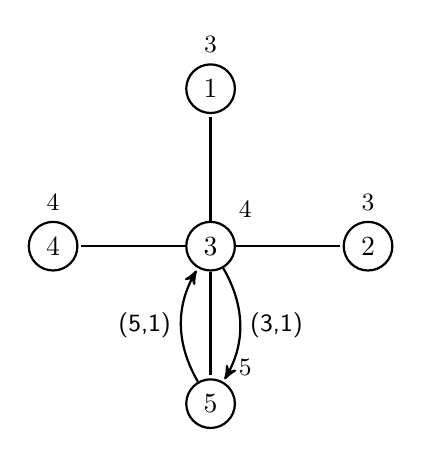
\begin{tikzpicture}[>=stealth',shorten >=1pt,auto,node distance=2cm,
                    thick,main node/.style={circle,draw,font=\normalsize}]
  \node[main node,label=above:{\small 3}] (1) {1};
  \node[main node,label=45:{\small 4}] (3) [below of=1] {3};
  \node[main node,label=above:{\small 3}] (2) [right of=3] {2};
  \node[main node,label=above:{\small 4}] (4) [left  of=3] {4};
  \node[main node,label=45:{\small 5}] (5) [below of=3] {5};
  \path[every node/.style={font=\sffamily\small}] 
    (5) edge [->,bend left] node [left] {(5,1)} (3)
    (3) edge [->,bend left] node [right] {(3,1)} (5)
    (3) edge node {} (1)
    (3) edge node {} (2)
    (3) edge node {} (4)
    (3) edge node {} (5)
    ;
\end{tikzpicture}
\end{column}
\vrule{}
\hspace*{10pt}
\begin{column}{.4\textwidth}
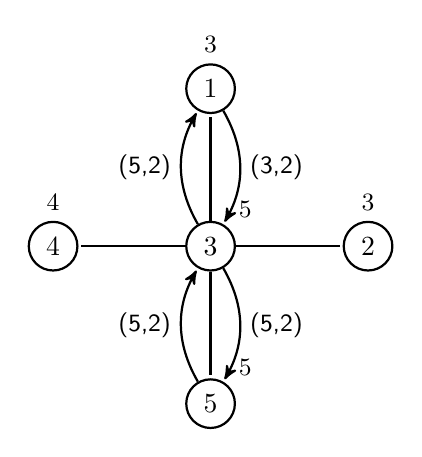
\begin{tikzpicture}[>=stealth',shorten >=1pt,auto,node distance=2cm,
                    thick,main node/.style={circle,draw,font=\normalsize}]
  \node[main node,label=above:{\small 3}] (1) {1};
  \node[main node,label=45:{\small 5}] (3) [below of=1] {3};
  \node[main node,label=above:{\small 3}] (2) [right of=3] {2};
  \node[main node,label=above:{\small 4}] (4) [left  of=3] {4};
  \node[main node,label=45:{\small 5}] (5) [below of=3] {5};
  \path[every node/.style={font=\sffamily\small}] 
    (5) edge [->,bend left] node [left] {(5,2)} (3)
    (3) edge [->,bend left] node [right] {(5,2)} (5)
    (1) edge [->,bend left] node [right] {(3,2)} (3)
    (3) edge [->,bend left] node [left] {(5,2)} (1)
    (3) edge node {} (1)
    (3) edge node {} (2)
    (3) edge node {} (4)
    (3) edge node {} (5)
    ;
\end{tikzpicture}
\end{column}
\end{columns}
\end{frame}

\begin{frame}{Asynchronous Floodmax}{Simulation (3 of 3)}
\begin{columns}
\begin{column}{.4\textwidth}
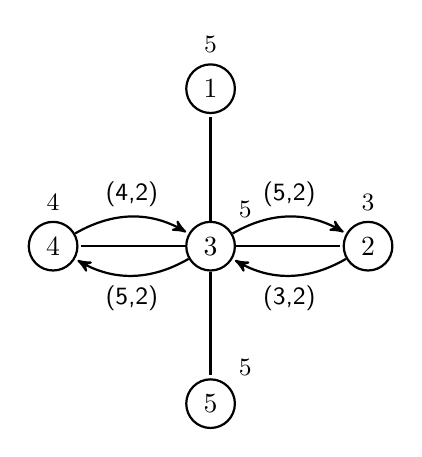
\begin{tikzpicture}[>=stealth',shorten >=1pt,auto,node distance=2cm,
                    thick,main node/.style={circle,draw,font=\normalsize}]
  \node[main node,label=above:{\small 5}] (1) {1};
  \node[main node,label=45:{\small 5}] (3) [below of=1] {3};
  \node[main node,label=above:{\small 3}] (2) [right of=3] {2};
  \node[main node,label=above:{\small 4}] (4) [left  of=3] {4};
  \node[main node,label=45:{\small 5}] (5) [below of=3] {5};
  \path[every node/.style={font=\sffamily\small}] 
    (4) edge [->,bend left] node [above] {(4,2)} (3)
    (3) edge [->,bend left] node [below] {(5,2)} (4)
    (2) edge [->,bend left] node [below] {(3,2)} (3)
    (3) edge [->,bend left] node [above] {(5,2)} (2)
    (3) edge node {} (1)
    (3) edge node {} (2)
    (3) edge node {} (4)
    (3) edge node {} (5)
    ;
\end{tikzpicture}
\end{column}
\vrule{}
\hspace*{10pt}
\begin{column}{.4\textwidth}
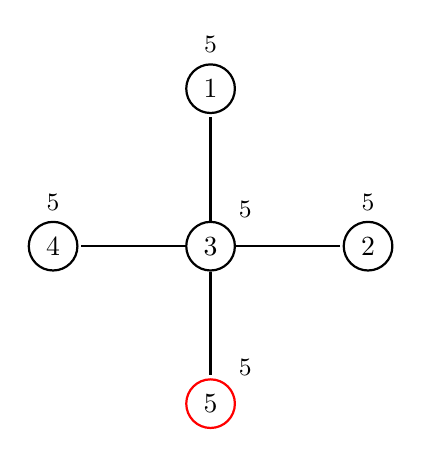
\begin{tikzpicture}[>=stealth',shorten >=1pt,auto,node distance=2cm,
                    thick,main node/.style={circle,draw,font=\normalsize}]
  \node[main node,label=above:{\small 5}] (1) {1};
  \node[main node,label=45:{\small 5}] (3) [below of=1] {3};
  \node[main node,label=above:{\small 5}] (2) [right of=3] {2};
  \node[main node,label=above:{\small 5}] (4) [left  of=3] {4};
  \node[main node,label=45:{\small 5}, draw=red] (5) [below of=3] {5};
  \path[every node/.style={font=\sffamily\small}] 
    (3) edge node {} (1)
    (3) edge node {} (2)
    (3) edge node {} (4)
    (3) edge node {} (5)
    ;
\end{tikzpicture}
\end{column}
\end{columns}
\end{frame}

\begin{frame}{Asynchronous Floodmax}{OptFloodMax}
    Is there any better algorithm? \\
    \vspace{12pt}
    There is a simple optimization that can be used to reduce the number of messages sent. The processes can propagate the maximum UID only when they first learn about them, instead of doing so each round.
    \vspace{12pt}
    This optimization is called \textbf{OptFloodMax}. 
\end{frame}

\begin{frame}{Asynchronous Floodmax}{OptFloodMax}
    There are two ways to implement OptFloodMax in the asynchronous model:
    \begin{itemize}
        \item Round simulation, as in normal FloodMax
        \item Purely asynchronously. 
    \end{itemize}
\end{frame}

\begin{frame}{Asynchronous Floodmax}{OptFloodMax - Round Simulation}
    If simulating rounds, we have a \textbf{round transition} problem. \\
    \vspace{12pt}
    A single process cannot determine when it has received all messages for a round $r$, so it cannot tell when to perform its round $r+1$ transition. \\
\end{frame}

\begin{frame}{Asynchronous Floodmax}{OptFloodMax Simulation (1 of 3)}
\begin{center}
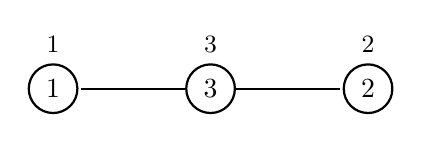
\begin{tikzpicture}[>=stealth',shorten >=1pt,auto,node distance=2cm,
                    thick,main node/.style={circle,draw,font=\normalsize}]
  \node[main node,label=above:{\small 1}] (1) {1};
  \node[main node,label=above:{\small 3}] (3) [right of=1] {3};
  \node[main node,label=above:{\small 2}] (2) [right of=3] {2};
  \path[every node/.style={font=\sffamily\small}] 
    (3) edge node {} (1)
    (3) edge node {} (2)
    ;
\end{tikzpicture}
\end{center}
\end{frame}

\begin{frame}{Asynchronous Floodmax}{OptFloodMax Simulation (2 of 3)}
\begin{center}
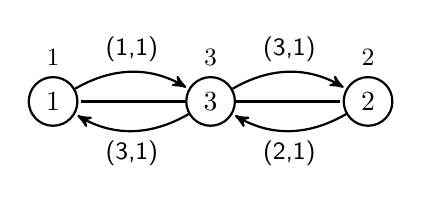
\begin{tikzpicture}[>=stealth',shorten >=1pt,auto,node distance=2cm,
                    thick,main node/.style={circle,draw,font=\normalsize}]
  \node[main node,label=above:{\small 1}] (1) {1};
  \node[main node,label=above:{\small 3}] (3) [right of=1] {3};
  \node[main node,label=above:{\small 2}] (2) [right of=3] {2};
  \path[every node/.style={font=\sffamily\small}] 
    (3) edge node {} (1)
    (3) edge node {} (2)
    (1) edge [->,bend left] node [above] {(1,1)} (3)
    (3) edge [->,bend left] node [below] {(3,1)} (1)
    (2) edge [->,bend left] node [below] {(2,1)} (3)
    (3) edge [->,bend left] node [above] {(3,1)} (2)
    ;
\end{tikzpicture}
\end{center}
\end{frame}

\begin{frame}{Asynchronous Floodmax}{OptFloodMax Simulation (3 of 3)}
\begin{center}
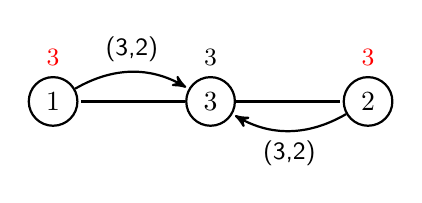
\begin{tikzpicture}[>=stealth',shorten >=1pt,auto,node distance=2cm,
                    thick,main node/.style={circle,draw,font=\normalsize}]
  \node[main node,label={[red]above:{\small 3}}] (1) {1};
  \node[main node,label={above:{\small 3}}] (3) [right of=1] {3};
  \node[main node,label={[red]above:{\small 3}}] (2) [right of=3] {2};
  \path[every node/.style={font=\sffamily\small}] 
    (3) edge node {} (1)
    (3) edge node {} (2)
    (1) edge [->,bend left] node [above] {(3,2)} (3)
    (2) edge [->,bend left] node [below] {(3,2)} (3)
    ;
\end{tikzpicture}
\end{center}
Since the nodes 1 and 2 do not receive the message for the round from 3, they never finish round 2. \\
\vspace{12pt}
\end{frame}

\begin{frame}{Asynchronous Floodmax}{OptFloodMax - Pure Asynchronous}
    The algorithm can be run purely asynchronously, without rounds: the processes will propagate UIDs only when they receive a greater one.\\
    \vspace{12pt}
    This strategy will eventually propagate the maximum.\\
    \vspace{12pt}
    However, the processes now \textbf{do not know when to terminate}.
\end{frame}

\begin{frame}{Leader Election - What can we do?}
    There are different solutions for electing a leader in the asynchronous model.\\
    \vspace{12pt}
    We'll be looking at the \emph{Asynchronous broadcast and convergecast, based on breadth-first search}.\\
    \vspace{12pt}
    To solve the leader election problem, we'll start from a spanning tree.
\end{frame}

\section{Spanning Tree}
\begin{frame}{Asynchronous Spanning Tree}{Why?}
    A spanning tree allows for a process to implement broadcast and convergecast on
    an arbitrary network.\\
    \vspace{12pt}
    \textbf{By having an unrooted spanning tree, we can also implement a leader election 
    easily.}
\end{frame}

\begin{frame}{STtoLeader}{Concept}
    \textbf{Assumptions}:
    \begin{itemize}
        \item Usage of convergecast; \\
        \item The network graph is undirected, with only local knowledge; \\
        \item The processes have UIDs; \\
        \item We have an unrooted spanning tree for the network.
    \end{itemize}
   
    \vspace{12pt}
    \textbf{Results}:
    A leader is elected for the network.
\end{frame}

\begin{frame}{STtoLeader}{Concept}
    The algorithm uses a convergecast of \emph{elect} messages starting from the leaves.\\
    \begin{itemize}
        \item Each leaf node sends an \emph{elect} message to its single neighbor; \\
        \item Afterwards, all nodes that have received \emph{elect} messages from all their neighbors \emph{except one} send out an \emph{elect} message to that remaining neighbor
        \item If a process receives \emph{elect} messages on every channel before
            sending an \emph{elect} message itself, it elects itself as a leader; \\
        \item If two \emph{elect} messages are sent on some edge in both directions, then
            one of the two processes at the endpoints will elect itself as a leader, based 
            on some condition (e.g., larger UID). 
    \end{itemize}
\end{frame}

\begin{frame}{STtoLeader}{Example (1 of 6)}
    \begin{center}
        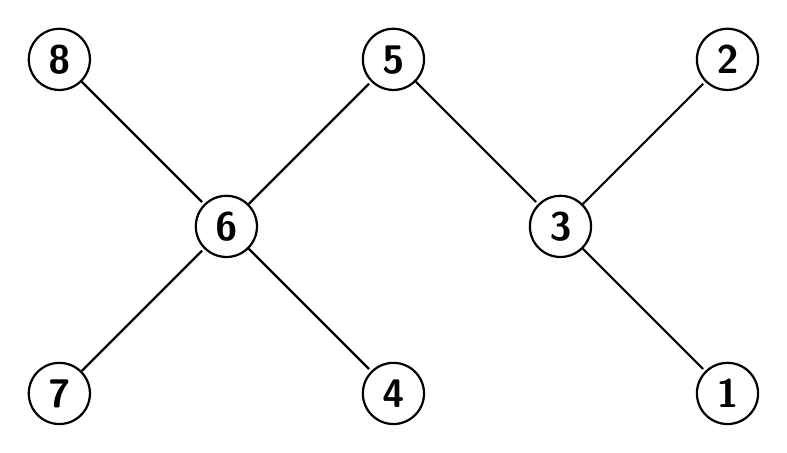
\begin{tikzpicture}[>=stealth',shorten >=1pt,auto,node distance=3cm,
        thick,main node/.style={circle,draw,font=\sffamily\Large\bfseries}]
            \node[main node] (6) [] {6};
            \node[main node] (8) [above left of=6] {8};
            \node[main node] (7) [below left of=6] {7};
            \node[main node] (5) [above right of=6] {5};
            \node[main node] (4) [below right of=6] {4};
            \node[main node] (3) [below right of=5] {3};
            \node[main node] (2) [above right of=3] {2};
            \node[main node] (1) [below right of=3] {1};
            \path[every node/.style={font=\sffamily\small}]
            (8) edge node [left] {} (6)
            (7) edge node [left] {} (6)
            (6) edge node [left] {} (5)
            (6) edge node [left] {} (4)
            (5) edge node [left] {} (3)
            (3) edge node [left] {} (2)
            (3) edge node [left] {} (1)
            ;
        \end{tikzpicture}
    \end{center}
\end{frame}

\begin{frame}{STtoLeader}{Example (2 of 6)}
    \begin{center}
        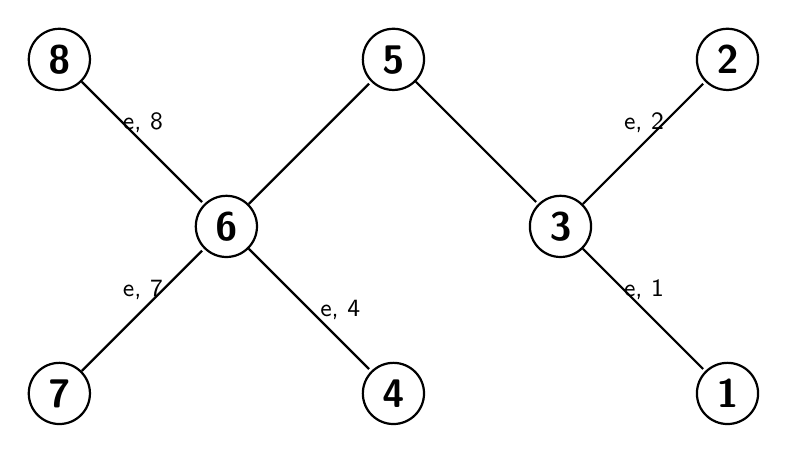
\begin{tikzpicture}[>=stealth',shorten >=1pt,auto,node distance=3cm,
        thick,main node/.style={circle,draw,font=\sffamily\Large\bfseries}]
        \node[main node] (6) [] {6};
        \node[main node] (8) [above left of=6] {8};
        \node[main node] (7) [below left of=6] {7};
        \node[main node] (5) [above right of=6] {5};
        \node[main node] (4) [below right of=6] {4};
        \node[main node] (3) [below right of=5] {3};
        \node[main node] (2) [above right of=3] {2};
        \node[main node] (1) [below right of=3] {1};
        \path[every node/.style={font=\sffamily\small}]
        (8) edge node [above] {e, 8} (6)
        (7) edge node [above] {e, 7} (6)
        (6) edge node [left] {} (5)
        (6) edge node [right] {e, 4} (4)
        (5) edge node [left] {} (3)
        (3) edge node [above] {e, 2} (2)
        (3) edge node [above] {e, 1} (1)
        ;
        \end{tikzpicture}
    \end{center}
\end{frame}

\begin{frame}{STtoLeader}{Example (3 of 6)}
    \begin{center}
        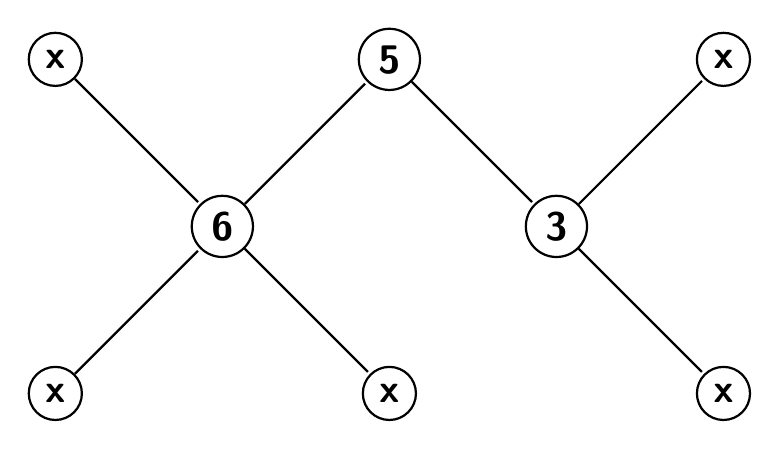
\begin{tikzpicture}[>=stealth',shorten >=1pt,auto,node distance=3cm,
        thick,main node/.style={circle,draw,font=\sffamily\Large\bfseries}]
        \node[main node] (6) [] {6};
        \node[main node] (8) [above left of=6] {x};
        \node[main node] (7) [below left of=6] {x};
        \node[main node] (5) [above right of=6] {5};
        \node[main node] (4) [below right of=6] {x};
        \node[main node] (3) [below right of=5] {3};
        \node[main node] (2) [above right of=3] {x};
        \node[main node] (1) [below right of=3] {x};
        \path[every node/.style={font=\sffamily\small}]
        (8) edge node [above] {} (6)
        (7) edge node [above] {} (6)
        (6) edge node [left] {} (5)
        (6) edge node [right] {} (4)
        (5) edge node [left] {} (3)
        (3) edge node [above] {} (2)
        (3) edge node [above] {} (1)
        ;
        \end{tikzpicture}
    \end{center}
\end{frame}

\begin{frame}{STtoLeader}{Example (4 of 6)}
    \begin{center}
        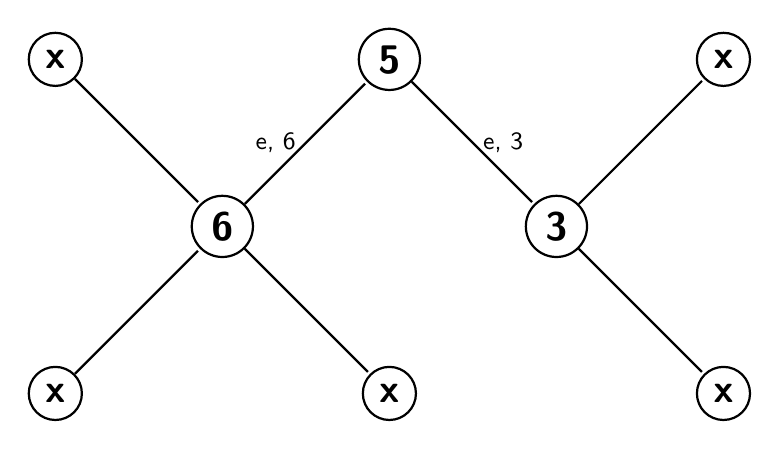
\begin{tikzpicture}[>=stealth',shorten >=1pt,auto,node distance=3cm,
        thick,main node/.style={circle,draw,font=\sffamily\Large\bfseries}]
        \node[main node] (6) [] {6};
        \node[main node] (8) [above left of=6] {x};
        \node[main node] (7) [below left of=6] {x};
        \node[main node] (5) [above right of=6] {5};
        \node[main node] (4) [below right of=6] {x};
        \node[main node] (3) [below right of=5] {3};
        \node[main node] (2) [above right of=3] {x};
        \node[main node] (1) [below right of=3] {x};
        \path[every node/.style={font=\sffamily\small}]
        (8) edge node [above] {} (6)
        (7) edge node [above] {} (6)
        (6) edge node [left] {e, 6} (5)
        (6) edge node [right] {} (4)
        (5) edge node [right] {e, 3} (3)
        (3) edge node [above] {} (2)
        (3) edge node [above] {} (1)
        ;
        \end{tikzpicture}
    \end{center}
\end{frame}

\begin{frame}{STtoLeader}{Example (5 of 6)}
    \begin{center}
        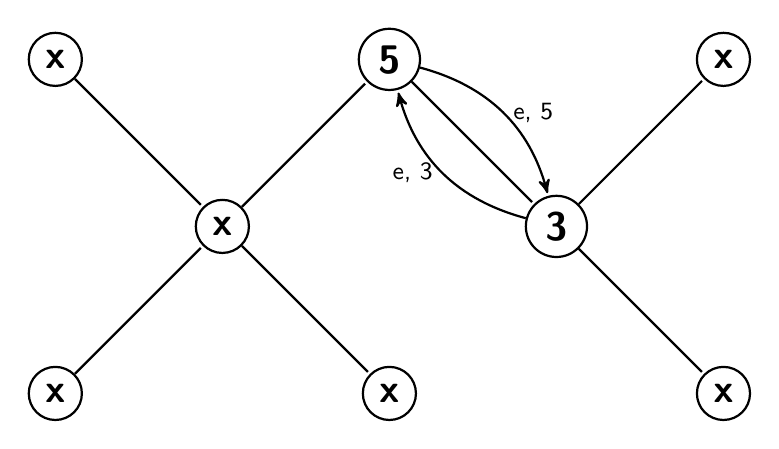
\begin{tikzpicture}[>=stealth',shorten >=1pt,auto,node distance=3cm,
        thick,main node/.style={circle,draw,font=\sffamily\Large\bfseries}]
        \node[main node] (6) [] {x};
        \node[main node] (8) [above left of=6] {x};
        \node[main node] (7) [below left of=6] {x};
        \node[main node] (5) [above right of=6] {5};
        \node[main node] (4) [below right of=6] {x};
        \node[main node] (3) [below right of=5] {3};
        \node[main node] (2) [above right of=3] {x};
        \node[main node] (1) [below right of=3] {x};
        \path[every node/.style={font=\sffamily\small}]
        (8) edge node [above] {} (6)
        (7) edge node [above] {} (6)
        (6) edge node [left] {} (5)
        (6) edge node [right] {} (4)
        (3) edge [->, bend left] node [left] {e, 3} (5)
        (5) edge [->, bend left] node [right] {e, 5} (3)
        (5) edge node [right] {} (3)
        (3) edge node [above] {} (2)
        (3) edge node [above] {} (1)
        ;
        \end{tikzpicture}
    \end{center}
\end{frame}

\begin{frame}{STtoLeader}{Example (6 of 6)}
    \begin{center}
        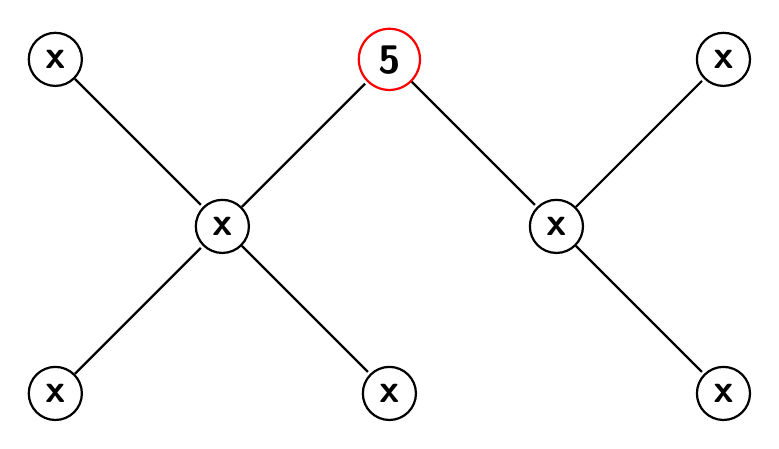
\begin{tikzpicture}[>=stealth',shorten >=1pt,auto,node distance=3cm,
        thick,main node/.style={circle,draw,font=\sffamily\Large\bfseries}]
        \node[main node] (6) [] {x};
        \node[main node] (8) [above left of=6] {x};
        \node[main node] (7) [below left of=6] {x};
        \node[main node] (5) [above right of=6, draw=red] {5};
        \node[main node] (4) [below right of=6] {x};
        \node[main node] (3) [below right of=5] {x};
        \node[main node] (2) [above right of=3] {x};
        \node[main node] (1) [below right of=3] {x};
        \path[every node/.style={font=\sffamily\small}]
        (8) edge node [above] {} (6)
        (7) edge node [above] {} (6)
        (6) edge node [left] {} (5)
        (6) edge node [right] {} (4)
        (5) edge node [right] {} (3)
        (3) edge node [above] {} (2)
        (3) edge node [above] {} (1)
        ;
        \end{tikzpicture}
    \end{center}
\end{frame}

\begin{frame}{Asynchronous Spanning Tree}{STtoLeader Results}
    Message complexity: \emph{n}.\\
    Time complexity: $\mathcal{O}(n*(l+d))$.\\
    \vspace{12pt}
    $n$ is the number of nodes in the graph.\\
    $l$ is the upper bound for each task in the process to be completed.
    $d$ is the upper bound for a message to be passed through the channel.
\end{frame}

\begin{frame}{Asynchronous Spanning Tree}{Base Algorithm}
    The \emph{AsynchSpanningTree} algorithm works on the premises:
    \begin{itemize}
        \item{The graph is undirected and connected.}
        \pause
        \item{There is a marked node $i_0$.}
    \end{itemize}
    \vspace{12pt}
    \pause
    Search messages start from $i_0$ and propagate throughout the network.\\
    \pause
    \vspace{12pt}
    A node receiving a search message from $i$, denotes $i$ as the parent, and
    propagates the search message to its neighbors.
\end{frame}

\begin{frame}{Asynchronous Spanning Tree}{Simulation (1 of 9)}
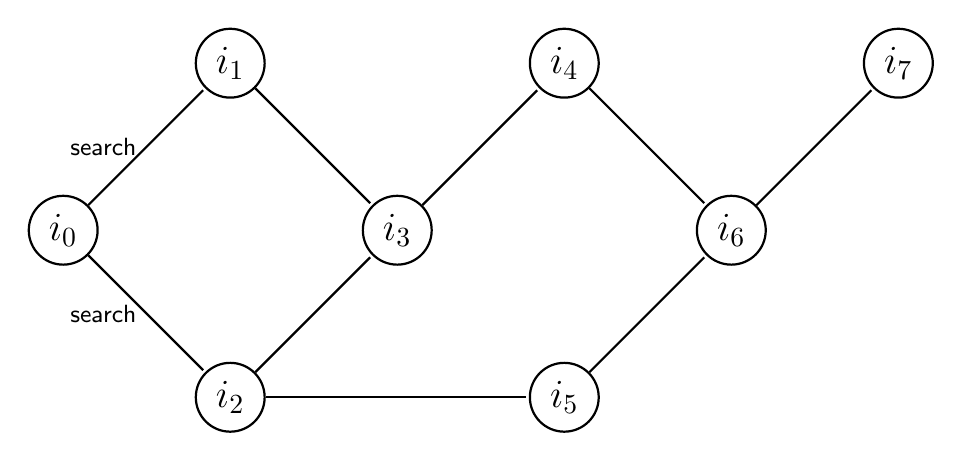
\begin{tikzpicture}[>=stealth',shorten >=1pt,auto,node distance=3cm,
                    thick,main node/.style={circle,draw,font=\sffamily\Large\bfseries}]
  \node[main node] (1) {$i_0$};
  \node[main node] (2) [above right of=1] {$i_1$};
  \node[main node] (3) [below right of=1] {$i_2$};
  \node[main node] (4) [below right of=2] {$i_3$};
  \node[main node] (5) [above right of=4] {$i_4$};
  \node[main node] (6) [below right of=4] {$i_5$};
  \node[main node] (7) [above right of=6] {$i_6$};
  \node[main node] (8) [above right of=7] {$i_7$};
  \path[every node/.style={font=\sffamily\small}]
    (1) edge node [left] {search} (2)
        edge node [left] {search} (3)
    (2) edge node [left] {} (4)
    (3) edge node [left] {} (4)
    (3) edge node [left] {} (6)
    (4) edge node [left] {} (5)
    (5) edge node [left] {} (7)
    (6) edge node [left] {} (7)
    (7) edge node [left] {} (8);
\end{tikzpicture}
\end{frame}

\begin{frame}{Asynchronous Spanning Tree}{Simulation (2 of 9)}
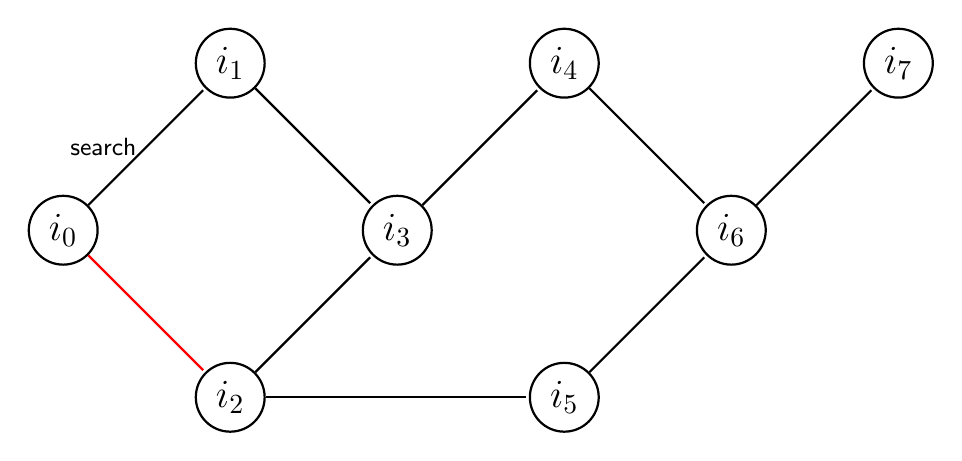
\begin{tikzpicture}[>=stealth',shorten >=1pt,auto,node distance=3cm,
                    thick,main node/.style={circle,draw,font=\sffamily\Large\bfseries}]
  \node[main node] (1) {$i_0$};
  \node[main node] (2) [above right of=1] {$i_1$};
  \node[main node] (3) [below right of=1] {$i_2$};
  \node[main node] (4) [below right of=2] {$i_3$};
  \node[main node] (5) [above right of=4] {$i_4$};
  \node[main node] (6) [below right of=4] {$i_5$};
  \node[main node] (7) [above right of=6] {$i_6$};
  \node[main node] (8) [above right of=7] {$i_7$};
  \path[every node/.style={font=\sffamily\small}]
    (1) edge node [left] {search} (2)
        edge [draw=red] node [left] {} (3)
    (2) edge node [left] {} (4)
    (3) edge node [left] {} (4)
    (3) edge node [left] {} (6)
    (4) edge node [left] {} (5)
    (5) edge node [left] {} (7)
    (6) edge node [left] {} (7)
    (7) edge node [left] {} (8);
\end{tikzpicture}
\end{frame}

\begin{frame}{Asynchronous Spanning Tree}{Simulation (3 of 9)}
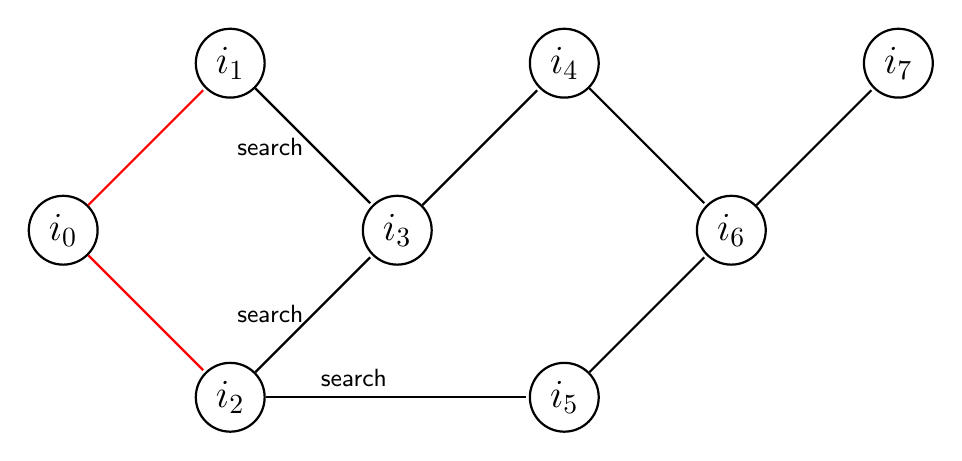
\begin{tikzpicture}[>=stealth',shorten >=1pt,auto,node distance=3cm,
                    thick,main node/.style={circle,draw,font=\sffamily\Large\bfseries}]
  \node[main node] (1) {$i_0$};
  \node[main node] (2) [above right of=1] {$i_1$};
  \node[main node] (3) [below right of=1] {$i_2$};
  \node[main node] (4) [below right of=2] {$i_3$};
  \node[main node] (5) [above right of=4] {$i_4$};
  \node[main node] (6) [below right of=4] {$i_5$};
  \node[main node] (7) [above right of=6] {$i_6$};
  \node[main node] (8) [above right of=7] {$i_7$};
  \path[every node/.style={font=\sffamily\small}]
    (1) edge [draw=red] node [left] {} (2)
        edge [draw=red] node [left] {} (3)
    (2) edge node [left] {search} (4)
    (3) edge node [left] {search} (4)
    (3) edge node [above left] {search} (6)
    (4) edge node [left] {} (5)
    (5) edge node [left] {} (7)
    (6) edge node [left] {} (7)
    (7) edge node [left] {} (8);
\end{tikzpicture}
\end{frame}

\begin{frame}{Asynchronous Spanning Tree}{Simulation (4 of 9)}
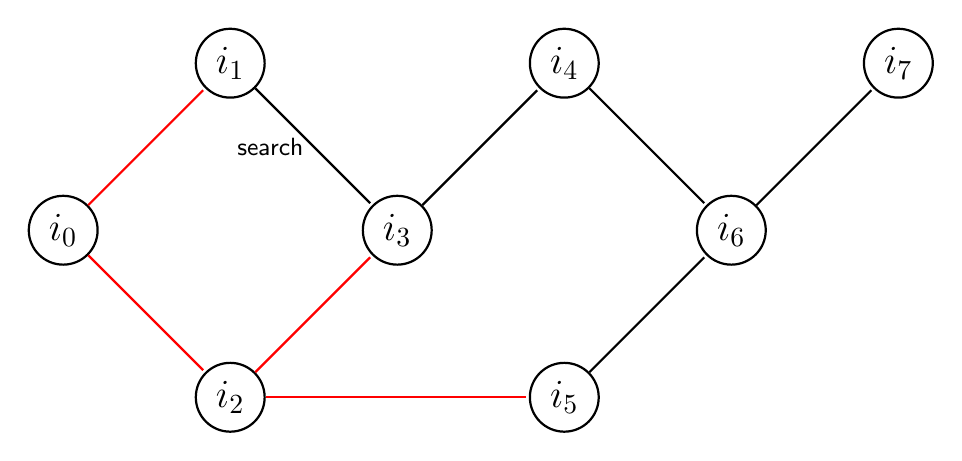
\begin{tikzpicture}[>=stealth',shorten >=1pt,auto,node distance=3cm,
                    thick,main node/.style={circle,draw,font=\sffamily\Large\bfseries}]
  \node[main node] (1) {$i_0$};
  \node[main node] (2) [above right of=1] {$i_1$};
  \node[main node] (3) [below right of=1] {$i_2$};
  \node[main node] (4) [below right of=2] {$i_3$};
  \node[main node] (5) [above right of=4] {$i_4$};
  \node[main node] (6) [below right of=4] {$i_5$};
  \node[main node] (7) [above right of=6] {$i_6$};
  \node[main node] (8) [above right of=7] {$i_7$};
  \path[every node/.style={font=\sffamily\small}]
    (1) edge [draw=red] node [left] {} (2)
        edge [draw=red] node [left] {} (3)
    (2) edge node [left] {search} (4)
    (3) edge [draw=red] node [left] {} (4)
    (3) edge [draw=red] node [below left] {} (6)
    (4) edge node [left] {} (5)
    (5) edge node [left] {} (7)
    (6) edge node [left] {} (7)
    (7) edge node [left] {} (8);
\end{tikzpicture}
\end{frame}

\begin{frame}{Asynchronous Spanning Tree}{Simulation (5 of 9)}
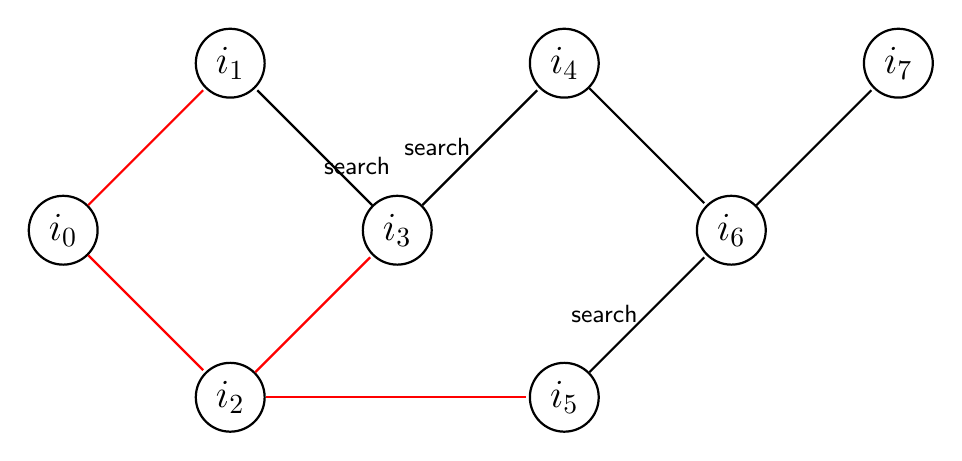
\begin{tikzpicture}[>=stealth',shorten >=1pt,auto,node distance=3cm,
                    thick,main node/.style={circle,draw,font=\sffamily\Large\bfseries}]
  \node[main node] (1) {$i_0$};
  \node[main node] (2) [above right of=1] {$i_1$};
  \node[main node] (3) [below right of=1] {$i_2$};
  \node[main node] (4) [below right of=2] {$i_3$};
  \node[main node] (5) [above right of=4] {$i_4$};
  \node[main node] (6) [below right of=4] {$i_5$};
  \node[main node] (7) [above right of=6] {$i_6$};
  \node[main node] (8) [above right of=7] {$i_7$};
  \path[every node/.style={font=\sffamily\small}]
    (1) edge [draw=red] node [left] {} (2)
        edge [draw=red] node [left] {} (3)
    (3) edge [draw=red] node [left] {} (4)
    (3) edge [draw=red] node [below left] {} (6)
    (4) edge [] node [below right] {search} (2)
    (4) edge node [left] {search} (5)
    (5) edge node [left] {} (7)
    (6) edge node [left] {search} (7)
    (7) edge node [left] {} (8);
\end{tikzpicture}
\end{frame}

\begin{frame}{Asynchronous Spanning Tree}{Simulation (6 of 9)}
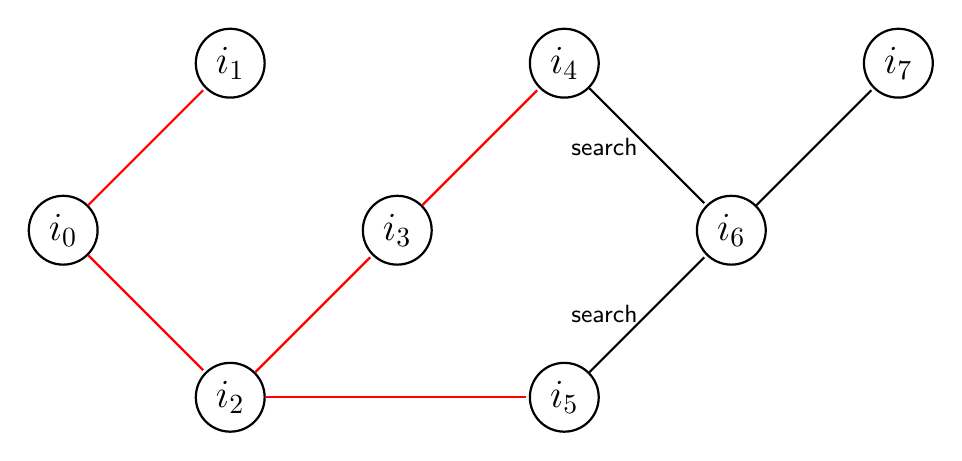
\begin{tikzpicture}[>=stealth',shorten >=1pt,auto,node distance=3cm,
                    thick,main node/.style={circle,draw,font=\sffamily\Large\bfseries}]
  \node[main node] (1) {$i_0$};
  \node[main node] (2) [above right of=1] {$i_1$};
  \node[main node] (3) [below right of=1] {$i_2$};
  \node[main node] (4) [below right of=2] {$i_3$};
  \node[main node] (5) [above right of=4] {$i_4$};
  \node[main node] (6) [below right of=4] {$i_5$};
  \node[main node] (7) [above right of=6] {$i_6$};
  \node[main node] (8) [above right of=7] {$i_7$};
  \path[every node/.style={font=\sffamily\small}]
    (1) edge [draw=red] node [left] {} (2)
        edge [draw=red] node [left] {} (3)
    (3) edge [draw=red] node [left] {} (4)
    (3) edge [draw=red] node [below left] {} (6)
    (4) edge [draw=red] node [left] {} (5)
    (5) edge node [left] {search} (7)
    (6) edge node [left] {search} (7)
    (7) edge node [left] {} (8);
\end{tikzpicture}
\end{frame}

\begin{frame}{Asynchronous Spanning Tree}{Simulation (7 of 9)}
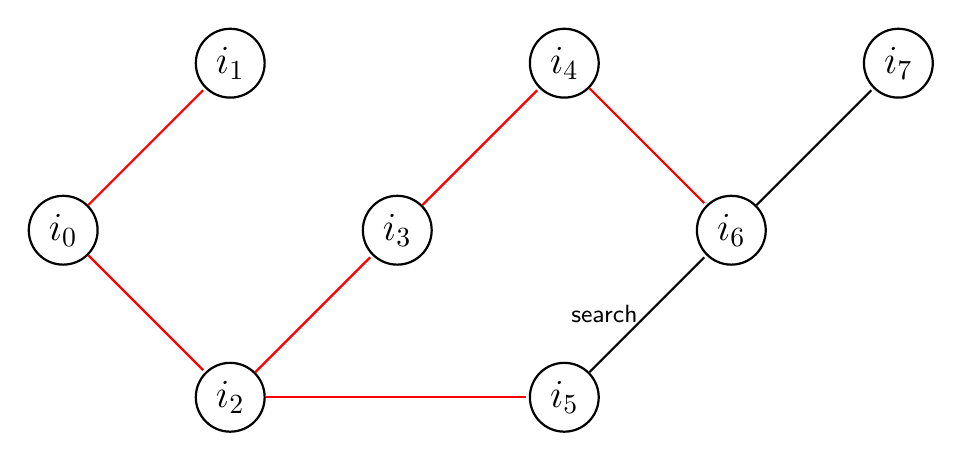
\begin{tikzpicture}[>=stealth',shorten >=1pt,auto,node distance=3cm,
                    thick,main node/.style={circle,draw,font=\sffamily\Large\bfseries}]
  \node[main node] (1) {$i_0$};
  \node[main node] (2) [above right of=1] {$i_1$};
  \node[main node] (3) [below right of=1] {$i_2$};
  \node[main node] (4) [below right of=2] {$i_3$};
  \node[main node] (5) [above right of=4] {$i_4$};
  \node[main node] (6) [below right of=4] {$i_5$};
  \node[main node] (7) [above right of=6] {$i_6$};
  \node[main node] (8) [above right of=7] {$i_7$};
  \path[every node/.style={font=\sffamily\small}]
    (1) edge [draw=red] node [left] {} (2)
        edge [draw=red] node [left] {} (3)
    (3) edge [draw=red] node [left] {} (4)
    (3) edge [draw=red] node [below left] {} (6)
    (4) edge [draw=red] node [left] {} (5)
    (5) edge [draw=red] node [left] {} (7)
    (6) edge node [left] {search} (7)
    (7) edge node [left] {} (8);
\end{tikzpicture}
\end{frame}

\begin{frame}{Asynchronous Spanning Tree}{Simulation (8 of 9)}
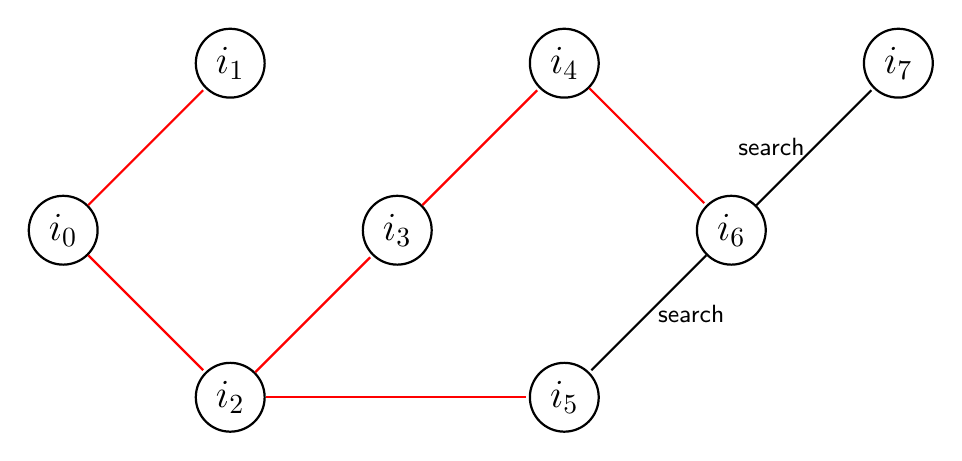
\begin{tikzpicture}[>=stealth',shorten >=1pt,auto,node distance=3cm,
                    thick,main node/.style={circle,draw,font=\sffamily\Large\bfseries}]
  \node[main node] (1) {$i_0$};
  \node[main node] (2) [above right of=1] {$i_1$};
  \node[main node] (3) [below right of=1] {$i_2$};
  \node[main node] (4) [below right of=2] {$i_3$};
  \node[main node] (5) [above right of=4] {$i_4$};
  \node[main node] (6) [below right of=4] {$i_5$};
  \node[main node] (7) [above right of=6] {$i_6$};
  \node[main node] (8) [above right of=7] {$i_7$};
  \path[every node/.style={font=\sffamily\small}]
    (1) edge [draw=red] node [left] {} (2)
        edge [draw=red] node [left] {} (3)
    (3) edge [draw=red] node [left] {} (4)
    (3) edge [draw=red] node [below left] {} (6)
    (4) edge [draw=red] node [left] {} (5)
    (5) edge [draw=red] node [left] {} (7)
    (7) edge [] node [right] {search} (6)
    (7) edge node [left] {search} (8);
\end{tikzpicture}
\end{frame}

\begin{frame}{Asynchronous Spanning Tree}{Simulation (9 of 9)}
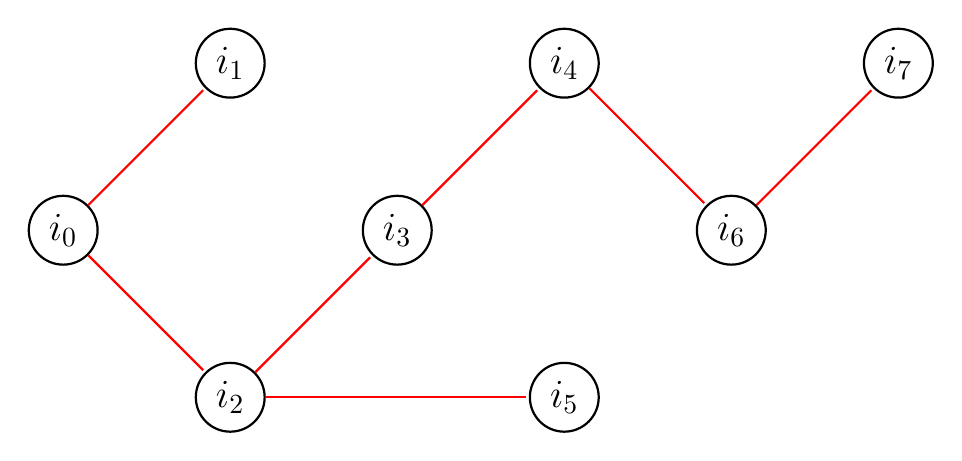
\begin{tikzpicture}[>=stealth',shorten >=1pt,auto,node distance=3cm,
                    thick,main node/.style={circle,draw,font=\sffamily\Large\bfseries}]
  \node[main node] (1) {$i_0$};
  \node[main node] (2) [above right of=1] {$i_1$};
  \node[main node] (3) [below right of=1] {$i_2$};
  \node[main node] (4) [below right of=2] {$i_3$};
  \node[main node] (5) [above right of=4] {$i_4$};
  \node[main node] (6) [below right of=4] {$i_5$};
  \node[main node] (7) [above right of=6] {$i_6$};
  \node[main node] (8) [above right of=7] {$i_7$};
  \path[every node/.style={font=\sffamily\small}]
    (1) edge [draw=red] node [left] {} (2)
        edge [draw=red] node [left] {} (3)
    (3) edge [draw=red] node [left] {} (4)
    (3) edge [draw=red] node [below left] {} (6)
    (4) edge [draw=red] node [left] {} (5)
    (5) edge [draw=red] node [left] {} (7)
    (7) edge [draw=red] node [left] {} (8);
\end{tikzpicture}
\end{frame}

\begin{frame}{Asynchronous Spanning Tree}{Algorithm}
	$AsynchSpanningTree_i$
    \begin{block}{Signature}
        \begin{columns}
            \column{.5\textwidth}
            Input:\\
            \hspace*{2pt} 
              {$receive("search")_{j,i}, j \in nbrs$}
            \column{.5\textwidth}
            Output:
            \hspace*{2pt}
            \parbox{\textwidth}{$send("search")_{i,j}, j \in nbrs$\\
               $parent(j)_i, j \in nbrs$}
        \end{columns}
    \end{block}
    \begin{block}{States}
        $parent \in nbrs \cup \{null\}$, initially $null$\\
        $reported$, a Boolean, initially $false$\\
        for every $j \in nbrs$:\\
        \hspace*{2pt}
        \parbox{\textwidth}{$send(j) \in \{search,null\}$,
        initially $search$ if $i=i_0$, else $null$}
    \end{block}
\end{frame}

\begin{frame}{Asynchronous Spanning Tree}{Algorithm}
    \begin{block}{Transitions}
        \begin{columns}[t]
            \column{.5\textwidth}
            $send("search")_{i,j}$ \\
            \hspace*{2pt} {Precondition:} \\
            \hspace*{5pt} {$send(j) = search$} \\
            \hspace*{2pt} {Effect:} \\
            \hspace*{5pt} {$send(j) := null$} \\
            \vspace{12pt}
            $receive("search")_{j,i}$ \\
            \hspace*{2pt} {Effect:} \\
            \hspace*{5pt} {if $i \neq i_0$ and $parent = null$ then}\\
            \hspace*{7pt} {$parent := j$} \\
            \hspace*{7pt} {for all $k \in nbrs - \{j\}$ do} \\
            \hspace*{9pt} {$send(k) := search$} 
            \column{.5\textwidth}
            $parent(j)_{i}$ \\
            \hspace*{2pt} {Precondition:} \\
            \hspace*{5pt} {$parent = j$} \\
            \hspace*{5pt} {$reported = false$} \\
            \hspace*{2pt} {Effect:} \\
            \hspace*{5pt} {$reported := true$} 
        \end{columns}
    \end{block}
    \vskip-3cm
    \begin{columns}
     \column{.5\textwidth}
    \column{.5\textwidth}
    \begin{block}{Tasks}
    $\{parent(j)_i : j \in nbrs\}$\\
    for every $j \in nbrs$: \\
        \hspace*{2pt}
        \parbox{\textwidth}{$\{send("search")_{i,j}\}$}
    \end{block}
    \end{columns}
\end{frame}

\begin{frame}[plain]{Asynchronous Spanning Tree}{Proof}
    \begin{block}{Assertion 1}
    In any reachable state, the edges defined by all the parent variables form a spanning tree
    of a subgraph of $G$, containing $i_0$; moreover, if there is a message in any channel $C_{i,j}$,
    then $i$ is in this spanning tree.
    \end{block}	
    \begin{block}{Assertion 2 - Liveness}
        In any reachable state, if $i=i_0$ or $parent_i \neq null$, and if $j \in nbrs_i - \{i_0\}$,
        then either $parent_j \neq null$ or $C_{i,j}$ contains a $search$ message or $send(j)_i$ contains a $search$ message.
    \end{block}	
    \begin{block}{Conclusions}
        From these two assertions we can then argue that the algorithm constructs a spanning tree.\\
        Furthermore, for any $i \neq i_0$ we have $parent_i \neq null$ within time $distance(i_0,i)\cdot(l+d)$, which implies the liveness.
    \end{block}
\end{frame}

\begin{frame}[plain]{Asynchronous Spanning Tree}{Proof}
    \begin{block}{Assertion 1}
    In any reachable state, the edges defined by all the parent variables form a spanning tree
    of a subgraph of $G$, containing $i_0$; moreover, if there is a message in any channel $C_{i,j}$,
    then $i$ is in this spanning tree.
    \end{block}	
    \pause
    \begin{block}{Proof - Base case}
    The first part is trivially proven,
    as there are no parent variables, and $G$ contains $i_0$ by definition.\\
    Second part, we have search messages starting only from $i_0$, by the algorithm definition.\\
    \end{block}
\end{frame}

\begin{frame}[plain]{Asynchronous Spanning Tree}{Proof}
    \begin{block}{Assertion 1}
    In any reachable state, the edges defined by all the parent variables form a spanning tree
    of a subgraph of $G$, containing $i_0$; moreover, if there is a message in any channel $C_{i,j}$,
    then $i$ is in this spanning tree.
    \end{block}	
    \begin{block}{Proof - Inductive step}
    We look at each transition, and how it does not change the invariant.
    \begin{columns}
    \begin{column}{.5\textwidth}
    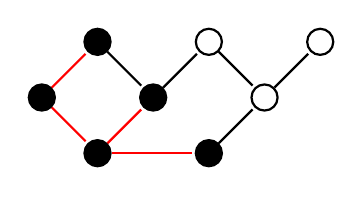
\begin{tikzpicture}[>=stealth',shorten >=1pt,auto,node distance=1cm,
                    thick,main node/.style={circle,draw,font=\small,minimum size=0.1cm}]
      \node[main node, fill=black] (1) {};
      \node[main node, fill=black] (2) [above right of=1] {};
      \node[main node, fill=black] (3) [below right of=1] {};
      \node[main node, fill=black] (4) [below right of=2] {};
      \node[main node] (5) [above right of=4] {};
      \node[main node, fill=black] (6) [below right of=4] {};
      \node[main node] (7) [above right of=6] {};
      \node[main node] (8) [above right of=7] {};
      \path[every node/.style={font=\sffamily\small}]
        (1) edge [draw=red] node [left] {} (2)
            edge [draw=red] node [left] {} (3)
        (3) edge [draw=red] node [left] {} (4)
        (2) edge [] node [left] {} (4)
        (3) edge [draw=red] node [below left] {} (6)
        (4) edge [] node [left] {} (5)
        (5) edge [] node [left] {} (7)
        (6) edge [] node [left] {} (7)
        (7) edge [] node [left] {} (8);
    \end{tikzpicture}
    \end{column}
    \hspace{-25pt}
    \begin{column}{.5\textwidth}
            $receive("search")_{j,i}$ \\
            \hspace*{2pt} {Effect:} \\
            \hspace*{5pt} {if $i \neq i_0$ and $parent = null$ then}\\
            \hspace*{7pt} {$parent := j$} \\
            \hspace*{7pt} {for all $k \in nbrs - \{j\}$ do} \\
            \hspace*{9pt} {$send(k) := search$} 
    \end{column}
    \end{columns}
    %\begin{description}
    %\item[$send$]{Since the send transition sends a message from the node i to the neighbors, we need
    %    to prove that i is in the spanning tree. By the algorithm, the send transition has the precondition of the $send(j)$ variable,
    %which is set only as the node enters the spanning tree.}
    %\end{description}
    \end{block}
\end{frame}

\begin{frame}[plain]{Asynchronous Spanning Tree}{Proof}
    \begin{block}{Assertion 1}
    In any reachable state, the edges defined by all the parent variables form a spanning tree
    of a subgraph of $G$, containing $i_0$; moreover, if there is a message in any channel $C_{i,j}$,
    then $i$ is in this spanning tree.
    \end{block}	
    \begin{block}{Proof - Inductive step}
    \begin{columns}
    \begin{column}{.5\textwidth}
    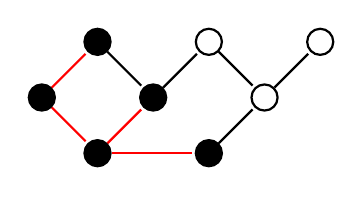
\begin{tikzpicture}[>=stealth',shorten >=1pt,auto,node distance=1cm,
                    thick,main node/.style={circle,draw,font=\small,minimum size=0.1cm}]
      \node[main node, fill=black] (1) {};
      \node[main node, fill=black] (2) [above right of=1] {};
      \node[main node, fill=black] (3) [below right of=1] {};
      \node[main node, fill=black] (4) [below right of=2] {};
      \node[main node] (5) [above right of=4] {};
      \node[main node, fill=black] (6) [below right of=4] {};
      \node[main node] (7) [above right of=6] {};
      \node[main node] (8) [above right of=7] {};
      \path[every node/.style={font=\sffamily\small}]
        (1) edge [draw=red] node [left] {} (2)
            edge [draw=red] node [left] {} (3)
        (3) edge [draw=red] node [left] {} (4)
        (2) edge [] node [left] {} (4)
        (3) edge [draw=red] node [below left] {} (6)
        (4) edge [] node [left] {} (5)
        (5) edge [] node [left] {} (7)
        (6) edge [] node [left] {} (7)
        (7) edge [] node [left] {} (8);
    \end{tikzpicture}
    \end{column}
    \begin{column}{.4\textwidth}
            $send("search")_{i,j}$ \\
            \hspace*{2pt} {Precondition:} \\
            \hspace*{5pt} {$send(j) = search$} \\
            \hspace*{2pt} {Effect:} \\
            \hspace*{5pt} {$send(j) := null$} \\
    \end{column}
    \end{columns}
    \end{block}

    %\begin{description}
    %\item[$receive$]{\small The receive of a search message to a node not in the spanning tree, allows for the node to enter the spanning tree by setting the parent variable to the neighbor that sent the message. It then sets the variables in order to send the search message to the remaining neighbors.\\
    %    If the node already has the parent variable set, it discards the message. 
    %Since this only adds a node, $i_0$ is still contained in the spanning tree.}
    %\end{description}
\end{frame}

\begin{frame}[plain]{Asynchronous Spanning Tree}{Proof}
    \begin{block}{Assertion 1}
    In any reachable state, the edges defined by all the parent variables form a spanning tree
    of a subgraph of $G$, containing $i_0$; moreover, if there is a message in any channel $C_{i,j}$,
    then $i$ is in this spanning tree.
    \end{block}	
    \begin{block}{Proof - Inductive step}
    \begin{columns}
    \begin{column}{.5\textwidth}
    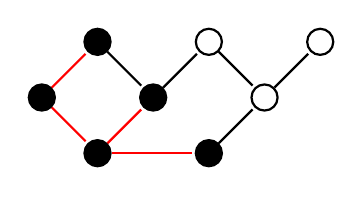
\begin{tikzpicture}[>=stealth',shorten >=1pt,auto,node distance=1cm,
                    thick,main node/.style={circle,draw,font=\small,minimum size=0.1cm}]
      \node[main node, fill=black] (1) {};
      \node[main node, fill=black] (2) [above right of=1] {};
      \node[main node, fill=black] (3) [below right of=1] {};
      \node[main node, fill=black] (4) [below right of=2] {};
      \node[main node] (5) [above right of=4] {};
      \node[main node, fill=black] (6) [below right of=4] {};
      \node[main node] (7) [above right of=6] {};
      \node[main node] (8) [above right of=7] {};
      \path[every node/.style={font=\sffamily\small}]
        (1) edge [draw=red] node [left] {} (2)
            edge [draw=red] node [left] {} (3)
        (3) edge [draw=red] node [left] {} (4)
        (2) edge [] node [left] {} (4)
        (3) edge [draw=red] node [below left] {} (6)
        (4) edge [] node [left] {} (5)
        (5) edge [] node [left] {} (7)
        (6) edge [] node [left] {} (7)
        (7) edge [] node [left] {} (8);
    \end{tikzpicture}
    \end{column}
    \begin{column}{.4\textwidth}
            $parent(j)_{i}$ \\
            \hspace*{2pt} {Precondition:} \\
            \hspace*{5pt} {$parent = j$} \\
            \hspace*{5pt} {$reported = false$} \\
            \hspace*{2pt} {Effect:} \\
            \hspace*{5pt} {$reported := true$} 
    \end{column}
    \end{columns}
    \end{block}
    %\begin{description}
    %\item[$parent$]{The parent action will activate once, as the parent variable is set, reporting the node's presence in the spanning tree.}
    %\end{description}
\end{frame}

\begin{frame}[plain]{Asynchronous Spanning Tree}{Proof}
    \begin{block}{Assertion 2 - Liveness}
        In any reachable state, if $i=i_0$ or $parent_i \neq null$, and if $j \in nbrs_i - \{i_0\}$,
        then either $parent_j \neq null$ or $C_{i,j}$ contains a $search$ message or $send(j)_i$ contains a $search$ message.
    \end{block}	
    \begin{block}{Proof - Base step}
    As the initial state, we have that every $parent_i = null$, so we need to only check $i_0$.
    As the initial state, $i_0$ has that for all its neighbors $send(j)_i$ contains a search message,
    therefore proving the invariant.
    \end{block}
\end{frame}
\begin{frame}[plain]{Asynchronous Spanning Tree}{Proof}
    \begin{block}{Assertion 2 - Liveness}
        In any reachable state, if $i=i_0$ or $parent_i \neq null$, and if $j \in nbrs_i - \{i_0\}$,
        then either $parent_j \neq null$ or $C_{i,j}$ contains a $search$ message or $send(j)_i$ contains a $search$ message.
    \end{block}	
    \begin{block}{Proof - Inductive step}
    We look at each transition, and show how it doesn't invalidate the invariant.
    \begin{columns}
    \begin{column}{.5\textwidth}
    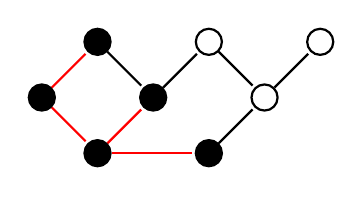
\begin{tikzpicture}[>=stealth',shorten >=1pt,auto,node distance=1cm,
                    thick,main node/.style={circle,draw,font=\small,minimum size=0.1cm}]
      \node[main node, fill=black] (1) {};
      \node[main node, fill=black] (2) [above right of=1] {};
      \node[main node, fill=black] (3) [below right of=1] {};
      \node[main node, fill=black] (4) [below right of=2] {};
      \node[main node] (5) [above right of=4] {};
      \node[main node, fill=black] (6) [below right of=4] {};
      \node[main node] (7) [above right of=6] {};
      \node[main node] (8) [above right of=7] {};
      \path[every node/.style={font=\sffamily\small}]
        (1) edge [draw=red] node [left] {} (2)
            edge [draw=red] node [left] {} (3)
        (3) edge [draw=red] node [left] {} (4)
        (2) edge [] node [left] {} (4)
        (3) edge [draw=red] node [below left] {} (6)
        (4) edge [] node [left] {} (5)
        (5) edge [] node [left] {} (7)
        (6) edge [] node [left] {} (7)
        (7) edge [] node [left] {} (8);
    \end{tikzpicture}
    \end{column}
    \begin{column}{.4\textwidth}
            $send("search")_{i,j}$ \\
            \hspace*{2pt} {Precondition:} \\
            \hspace*{5pt} {$send(j) = search$} \\
            \hspace*{2pt} {Effect:} \\
            \hspace*{5pt} {$send(j) := null$} \\
    \end{column}
    \end{columns}
    %\begin{description}
    %\item[$send$]{As the effect will remove the $search$ message from the $send(j)$ variable, the channel $C_{i,j}$ will now contain a $search$ message instead.}
    %\end{description}
    \end{block}
\end{frame}
\begin{frame}[plain]{Asynchronous Spanning Tree}{Proof}
    \begin{block}{Assertion 2 - Liveness}
        In any reachable state, if $i=i_0$ or $parent_i \neq null$, and if $j \in nbrs_i - \{i_0\}$,
        then either $parent_j \neq null$ or $C_{i,j}$ contains a $search$ message or $send(j)_i$ contains a $search$ message.
    \end{block}	
    \begin{block}{Proof - Inductive step}
    \begin{columns}
    \begin{column}{.5\textwidth}
    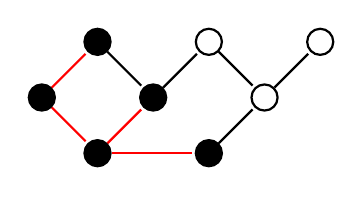
\begin{tikzpicture}[>=stealth',shorten >=1pt,auto,node distance=1cm,
                    thick,main node/.style={circle,draw,font=\small,minimum size=0.1cm}]
      \node[main node, fill=black] (1) {};
      \node[main node, fill=black] (2) [above right of=1] {};
      \node[main node, fill=black] (3) [below right of=1] {};
      \node[main node, fill=black] (4) [below right of=2] {};
      \node[main node] (5) [above right of=4] {};
      \node[main node, fill=black] (6) [below right of=4] {};
      \node[main node] (7) [above right of=6] {};
      \node[main node] (8) [above right of=7] {};
      \path[every node/.style={font=\sffamily\small}]
        (1) edge [draw=red] node [left] {} (2)
            edge [draw=red] node [left] {} (3)
        (3) edge [draw=red] node [left] {} (4)
        (2) edge [] node [left] {} (4)
        (3) edge [draw=red] node [below left] {} (6)
        (4) edge [] node [left] {} (5)
        (5) edge [] node [left] {} (7)
        (6) edge [] node [left] {} (7)
        (7) edge [] node [left] {} (8);
    \end{tikzpicture}
    \end{column}
    \hspace{-25pt}
    \begin{column}{.5\textwidth}
            $receive("search")_{j,i}$ \\
            \hspace*{2pt} {Effect:} \\
            \hspace*{5pt} {if $i \neq i_0$ and $parent = null$ then}\\
            \hspace*{7pt} {$parent := j$} \\
            \hspace*{7pt} {for all $k \in nbrs - \{j\}$ do} \\
            \hspace*{9pt} {$send(k) := search$} 
    \end{column}
    \end{columns}
    %\begin{description}
    %\item[$receive$]{As $parent_i$ becomes different than $null$, for each $j \in nbrs - {parent_i}$,
    %it will set $send(j) = search$. For $parent_i$ instead, we can already prove from the first assertion that since a message came from $parent_i$ it must be in the spanning tree, and so its $parent$ variable different than $null$.}
    %\item[$parent$]{It doesn't affect any of the variables in the assertion.}
    %\end{description}
    \end{block}
\end{frame}

\begin{frame}[plain]{Asynchronous Spanning Tree}{Proof}
    \begin{block}{Assertion 2 - Liveness}
        In any reachable state, if $i=i_0$ or $parent_i \neq null$, and if $j \in nbrs_i - \{i_0\}$,
        then either $parent_j \neq null$ or $C_{i,j}$ contains a $search$ message or $send(j)_i$ contains a $search$ message.
    \end{block}	
    \begin{block}{Proof - Inductive step}
    \begin{columns}
    \begin{column}{.5\textwidth}
    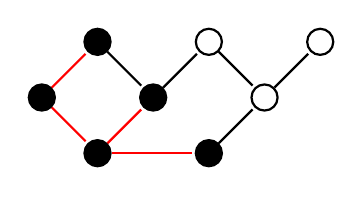
\begin{tikzpicture}[>=stealth',shorten >=1pt,auto,node distance=1cm,
                    thick,main node/.style={circle,draw,font=\small,minimum size=0.1cm}]
      \node[main node, fill=black] (1) {};
      \node[main node, fill=black] (2) [above right of=1] {};
      \node[main node, fill=black] (3) [below right of=1] {};
      \node[main node, fill=black] (4) [below right of=2] {};
      \node[main node] (5) [above right of=4] {};
      \node[main node, fill=black] (6) [below right of=4] {};
      \node[main node] (7) [above right of=6] {};
      \node[main node] (8) [above right of=7] {};
      \path[every node/.style={font=\sffamily\small}]
        (1) edge [draw=red] node [left] {} (2)
            edge [draw=red] node [left] {} (3)
        (3) edge [draw=red] node [left] {} (4)
        (2) edge [] node [left] {} (4)
        (3) edge [draw=red] node [below left] {} (6)
        (4) edge [] node [left] {} (5)
        (5) edge [] node [left] {} (7)
        (6) edge [] node [left] {} (7)
        (7) edge [] node [left] {} (8);
    \end{tikzpicture}
    \end{column}
    \hspace{-25pt}
    \begin{column}{.5\textwidth}
            $parent(j)_{i}$ \\
            \hspace*{2pt} {Precondition:} \\
            \hspace*{5pt} {$parent = j$} \\
            \hspace*{5pt} {$reported = false$} \\
            \hspace*{2pt} {Effect:} \\
            \hspace*{5pt} {$reported := true$} 
    \end{column}
    \end{columns}
    %\begin{description}
    %\item[$receive$]{As $parent_i$ becomes different than $null$, for each $j \in nbrs - {parent_i}$,
    %it will set $send(j) = search$. For $parent_i$ instead, we can already prove from the first assertion that since a message came from $parent_i$ it must be in the spanning tree, and so its $parent$ variable different than $null$.}
    %\item[$parent$]{It doesn't affect any of the variables in the assertion.}
    %\end{description}
    \end{block}
\end{frame}

\begin{frame}{Asynchronous Spanning Tree}{Results}
    Number of messages: $\mathcal{O}(|E|)$.\\
    Time upper bound for all processes except $i_0$: $diam(l+d)+l$.\\
    \vspace{6pt}
    $|E|$ is the number of edges in the graph.\\
    $n$ is the number of nodes in the graph.\\
    $l$ is the upper bound for each task in the process to be completed.\\
    $d$ is the upper bound for a message to be passed through the channel.\\
    \pause
    \vspace{6pt}
    The paths might be longer than the diameter, nonetheless the time is still bounded in 
    terms of diameter, because the time of the shortest path might be greater than the 
    fastest one.\\
    \pause
    \vspace{6pt}
    The algorithm does not actually know when to terminate.
\end{frame}

\begin{frame}{Asynchronous Spanning Tree}{Broadcast and Child Pointers}
    \begin{block}{Broadcast}
        It's easy to modify the algorithm, as we use a method of \emph{piggybacking} on the
        $search$ message. It also shares the complexities as the spanning tree algorithm.
    \end{block}
    \begin{block}{Child Pointers}
        Since the graph is assumed to be undirected, it's easy for the children to reply
        directly to the parent, in order for the parent to acknowledge them.\\
        The spanning tree with child pointers can also be used for \emph{convergecast}, with the same complexities as the broadcast.\\
        The two can be combined in a broadcast, followed by a convergecast to acknowledge the receival.\\
        Only with the child pointers modification the algorithm can terminate.
    \end{block}
\end{frame}

\section{Breadth-First Search}
\begin{frame}{Breadth-First Search}{Problem}
	Another way to build a Spanning Tree is via Breadth-First Search. \\
    \vspace{12pt}
    \pause
    \textbf{Requirements}:
    \begin{enumerate}
        \item An undirected, unweighted network graph; \pause
        \item A starting node $i_0$; \pause
    \end{enumerate}
    \vspace{12pt}
    \textbf{Result}: \\ \pause
    A breadth-first spanning tree for the network graph, in which all nodes are reached in the minimum amount of edges.
\end{frame}

\begin{frame}{Breadth-First Search}{Problem}
    There are various issues with the algorithm: \pause
    \begin{itemize}
        \item No guarantee that the nodes are reached along the shortest path at first. \pause $\to$ \textbf{The nodes have to be able to fix parent designations.} \pause
        \item \textbf{Termination} problem: if the nodes wait to be reached by shorter paths, they cannot know when to terminate. Even if a Breadth-First Spanning Tree is eventually built, the nodes will not be aware of it.
    \end{itemize}
\end{frame}

\begin{frame}{Breadth-First Search}{Algorithm}
	$AsynchBFS_i$
    \begin{block}{Signature}
        \begin{columns}
            \column{.5\textwidth}
            Input:\\
            \hspace*{\parindent} $receive(m)_{i,j}, m \in \mathbb{N}, j \in nbrs$
            \column{.5\textwidth}
            Output:
            \hspace*{\parindent} $send(m)_{i,j}, m \in \mathbb{N}, j \in nbrs$
        \end{columns}
    \end{block}
    \begin{block}{States}
        \begin{tcolorbox}[height=0.8cm,colframe=red]
        $dist \in \mathbb{N} \cup \{\infty\}$, initially $0$ if $i=i_0$, $\infty $ otherwise\\
        \end{tcolorbox}
        $parent \in nbrs \cup \{null\}$, initially $null$\\
        for every $j \in nbrs$:\\
        \hspace*{\parindent}
        \parbox{\textwidth}{$send(j)$,
        a FIFO queue of elements of $\mathbb{N}$,
        initially containing the single element $0$ if $i=i_0$, else $\emptyset$}
    \end{block}
	
\end{frame}

\begin{frame}{Breadth-First Search}{Algorithm}
	\begin{block}{Transitions}
        \vspace{2mm}
        \begin{columns}
            \column{.5\textwidth}
            $\mathbf{send(m)_{i, j}:}$\\ 
                \emph{Precondition}: \\ 
                \small $m$ is first on $send(j)$ \\
                \normalsize \emph{Effect}: \\
                \small remove first element of $send(j)$
            \column{.5\textwidth}
            \normalsize $\mathbf{receive(m)_{i, j}: }$ \\
                \emph{Effect}: \\
                \small
                \begin{tcolorbox}[colframe=red]
                    if $m+1 < dist$ then \\
                    \hspace*{\parindent} $dist := m+1$ \\
                    \hspace*{\parindent} $parent = j$ \\
                    \hspace*{\parindent} for all $k \in nbrs - \{j\}$ do \\
                    \hspace*{\parindent} \hspace*{\parindent} add $dist$ to $send(k)$ \\
                \end{tcolorbox}
        \end{columns}
	\end{block}
\end{frame}

\begin{frame}{AsynchBFS}{Simulation (1 of 8)}
    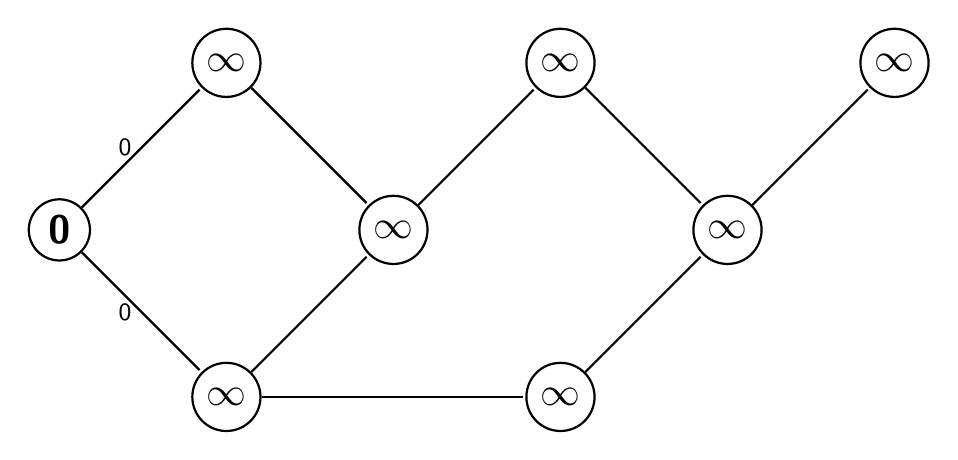
\begin{tikzpicture}[>=stealth',shorten >=1pt,auto,node distance=3cm,
    thick,main node/.style={circle,draw,font=\sffamily\Large\bfseries}]
    \node[main node] (1) {0};
    \node[main node] (2) [above right of=1] {$\infty$};
    \node[main node] (3) [below right of=1] {$\infty$};
    \node[main node] (4) [below right of=2] {$\infty$};
    \node[main node] (5) [above right of=4] {$\infty$};
    \node[main node] (6) [below right of=4] {$\infty$};
    \node[main node] (7) [above right of=6] {$\infty$};
    \node[main node] (8) [above right of=7] {$\infty$};
    \path[every node/.style={font=\sffamily\small}]
    (1) edge node [left] {0} (2)
    edge node [left] {0} (3)
    (2) edge node [left] {} (4)
    (3) edge node [left] {} (4)
    (3) edge node [left] {} (6)
    (4) edge node [left] {} (5)
    (5) edge node [left] {} (7)
    (6) edge node [left] {} (7)
    (7) edge node [left] {} (8);
    \end{tikzpicture}
\end{frame}

\begin{frame}{AsynchBFS}{Simulation (2 of 8)}
    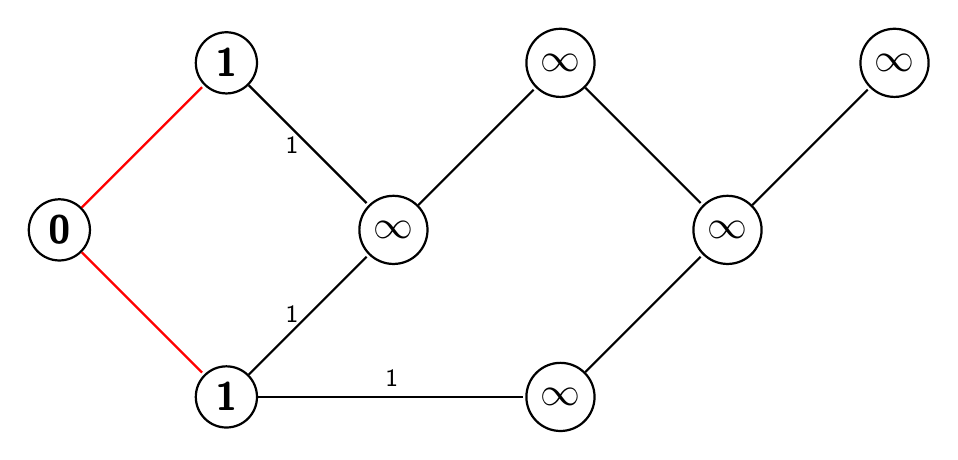
\begin{tikzpicture}[>=stealth',shorten >=1pt,auto,node distance=3cm,
    thick,main node/.style={circle,draw,font=\sffamily\Large\bfseries}]
    \node[main node] (1) {0};
    \node[main node] (2) [above right of=1] {1};
    \node[main node] (3) [below right of=1] {1};
    \node[main node] (4) [below right of=2] {$\infty$};
    \node[main node] (5) [above right of=4] {$\infty$};
    \node[main node] (6) [below right of=4] {$\infty$};
    \node[main node] (7) [above right of=6] {$\infty$};
    \node[main node] (8) [above right of=7] {$\infty$};
    \path[every node/.style={font=\sffamily\small}]
    (1) edge [draw=red] node [left] {} (2)
    (1) edge [draw=red] node [left] {} (3)
    (2) edge node [left] {1} (4)
    (3) edge node [left] {1} (4)
    (3) edge node [above] {1} (6)
    (4) edge node [left] {} (5)
    (5) edge node [left] {} (7)
    (6) edge node [left] {} (7)
    (7) edge node [left] {} (8);
    \end{tikzpicture}
\end{frame}

\begin{frame}{AsynchBFS}{Simulation (3 of 8)}
    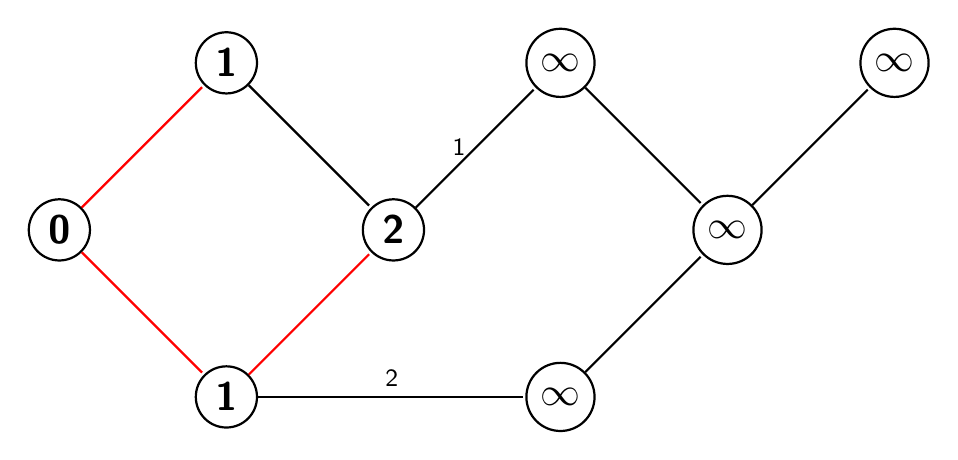
\begin{tikzpicture}[>=stealth',shorten >=1pt,auto,node distance=3cm,
    thick,main node/.style={circle,draw,font=\sffamily\Large\bfseries}]
    \node[main node] (1) {0};
    \node[main node] (2) [above right of=1] {1};
    \node[main node] (3) [below right of=1] {1};
    \node[main node] (4) [below right of=2] {2};
    \node[main node] (5) [above right of=4] {$\infty$};
    \node[main node] (6) [below right of=4] {$\infty$};
    \node[main node] (7) [above right of=6] {$\infty$};
    \node[main node] (8) [above right of=7] {$\infty$};
    \path[every node/.style={font=\sffamily\small}]
    (1) edge [draw=red] node [left] {} (2)
    edge [draw=red] node [left] {} (3)
    (2) edge node [left] {} (4)
    (3) edge [draw=red] node [left] {} (4)
    (3) edge node [above] {2} (6)
    (4) edge node [left] {1} (5)
    (5) edge node [left] {} (7)
    (6) edge node [left] {} (7)
    (7) edge node [left] {} (8);
    \end{tikzpicture}
\end{frame}

\begin{frame}{AsynchBFS}{Simulation (4 of 8)}
    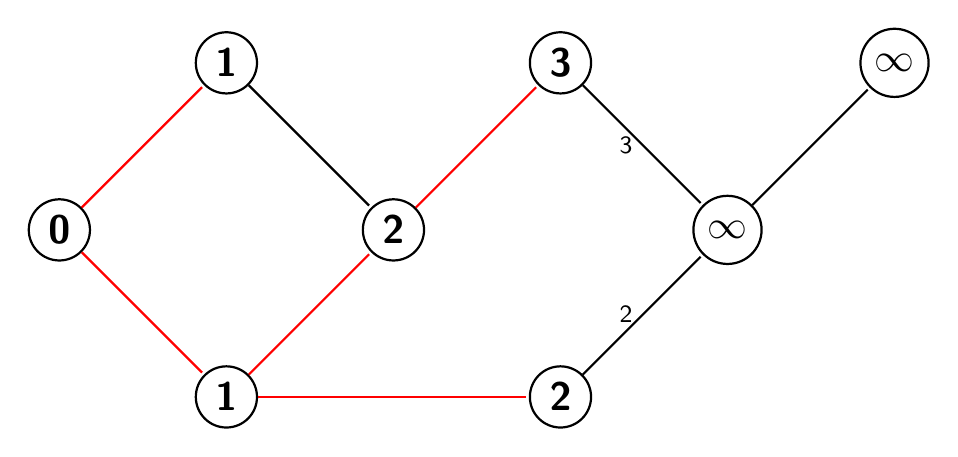
\begin{tikzpicture}[>=stealth',shorten >=1pt,auto,node distance=3cm,
    thick,main node/.style={circle,draw,font=\sffamily\Large\bfseries}]
    \node[main node] (1) {0};
    \node[main node] (2) [above right of=1] {1};
    \node[main node] (3) [below right of=1] {1};
    \node[main node] (4) [below right of=2] {2};
    \node[main node] (5) [above right of=4] {3};
    \node[main node] (6) [below right of=4] {2};
    \node[main node] (7) [above right of=6] {$\infty$};
    \node[main node] (8) [above right of=7] {$\infty$};
    \path[every node/.style={font=\sffamily\small}]
    (1) edge [draw=red] node [left] {} (2)
    edge [draw=red] node [left] {} (3)
    (2) edge node [left] {} (4)
    (3) edge [draw=red] node [left] {} (4)
    (3) edge [draw=red] node [below left] {} (6)
    (4) edge [draw=red] node [left] {} (5)
    (5) edge node [left] {3} (7)
    (6) edge node [left] {2} (7)
    (7) edge node [left] {} (8);
    \end{tikzpicture}
\end{frame}

\begin{frame}{AsynchBFS}{Simulation (5 of 8)}
    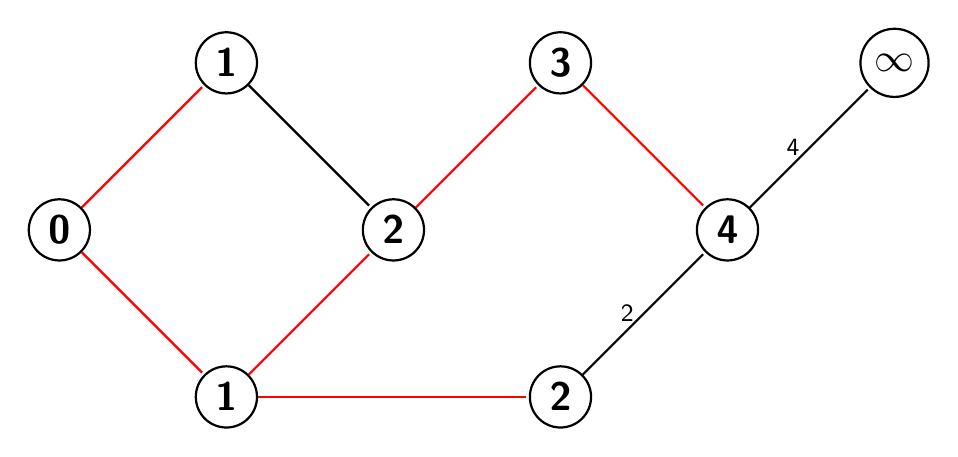
\begin{tikzpicture}[>=stealth',shorten >=1pt,auto,node distance=3cm,
    thick,main node/.style={circle,draw,font=\sffamily\Large\bfseries}]
    \node[main node] (1) {0};
    \node[main node] (2) [above right of=1] {1};
    \node[main node] (3) [below right of=1] {1};
    \node[main node] (4) [below right of=2] {2};
    \node[main node] (5) [above right of=4] {3};
    \node[main node] (6) [below right of=4] {2};
    \node[main node] (7) [above right of=6] {4};
    \node[main node] (8) [above right of=7] {$\infty$};
    \path[every node/.style={font=\sffamily\small}]
    (1) edge [draw=red] node [left] {} (2)
    edge [draw=red] node [left] {} (3)
    (2) edge node [left] {} (4)
    (3) edge [draw=red] node [left] {} (4)
    (3) edge [draw=red] node [below left] {} (6)
    (4) edge [draw=red] node [left] {} (5)
    (5) edge [draw=red] node [left] {} (7)
    (6) edge node [left] {2} (7)
    (7) edge node [left] {4} (8);
    \end{tikzpicture}
\end{frame}

\begin{frame}{AsynchBFS}{Simulation (6 of 8)}
    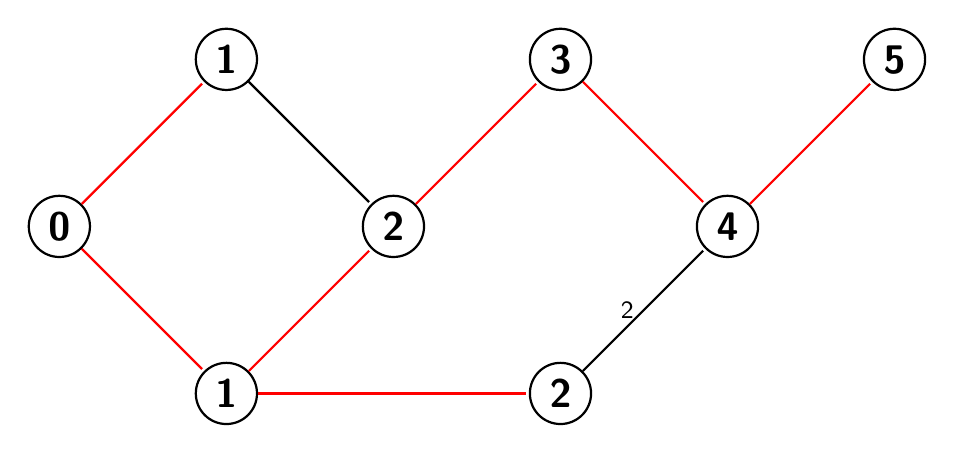
\begin{tikzpicture}[>=stealth',shorten >=1pt,auto,node distance=3cm,
    thick,main node/.style={circle,draw,font=\sffamily\Large\bfseries}]
    \node[main node] (1) {0};
    \node[main node] (2) [above right of=1] {1};
    \node[main node] (3) [below right of=1] {1};
    \node[main node] (4) [below right of=2] {2};
    \node[main node] (5) [above right of=4] {3};
    \node[main node] (6) [below right of=4] {2};
    \node[main node] (7) [above right of=6] {4};
    \node[main node] (8) [above right of=7] {5};
    \path[every node/.style={font=\sffamily\small}]
    (1) edge [draw=red] node [left] {} (2)
    edge [draw=red] node [left] {} (3)
    (2) edge node [left] {} (4)
    (3) edge [draw=red] node [left] {} (4)
    (3) edge [draw=red] node [below left] {} (6)
    (4) edge [draw=red] node [left] {} (5)
    (5) edge [draw=red] node [left] {} (7)
    (6) edge node [left] {2} (7)
    (7) edge [draw=red] node [left] {} (8);
    \end{tikzpicture}
\end{frame}

\begin{frame}{AsynchBFS}{Simulation (7 of 8)}
    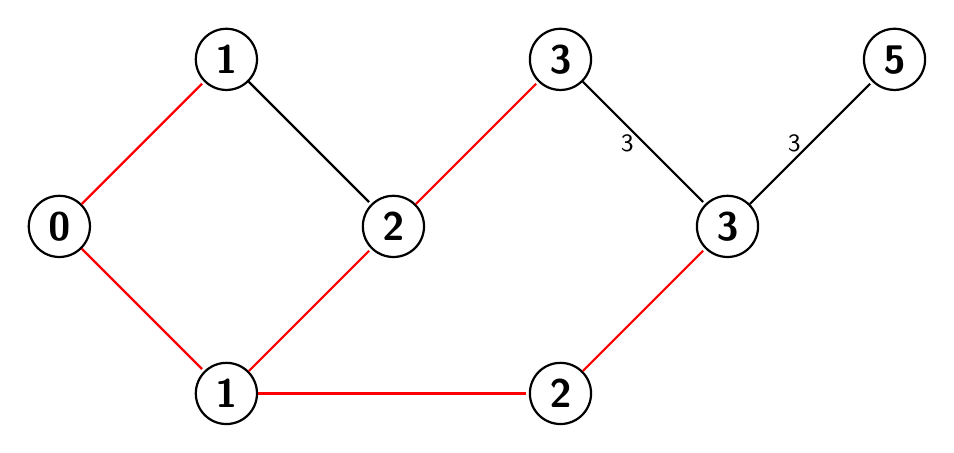
\begin{tikzpicture}[>=stealth',shorten >=1pt,auto,node distance=3cm,
    thick,main node/.style={circle,draw,font=\sffamily\Large\bfseries}]
    \node[main node] (1) {0};
    \node[main node] (2) [above right of=1] {1};
    \node[main node] (3) [below right of=1] {1};
    \node[main node] (4) [below right of=2] {2};
    \node[main node] (5) [above right of=4] {3};
    \node[main node] (6) [below right of=4] {2};
    \node[main node] (7) [above right of=6] {3};
    \node[main node] (8) [above right of=7] {5};
    \path[every node/.style={font=\sffamily\small}]
    (1) edge [draw=red] node [left] {} (2)
    edge [draw=red] node [left] {} (3)
    (2) edge node [left] {} (4)
    (3) edge [draw=red] node [left] {} (4)
    (3) edge [draw=red] node [below left] {} (6)
    (4) edge [draw=red] node [left] {} (5)
    (5) edge  node [left] {3} (7)
    (6) edge [draw=red] node [left] {} (7)
    (7) edge node [left] {3} (8);
    \end{tikzpicture}
\end{frame}

\begin{frame}{AsynchBFS}{Simulation (8 of 8)}
    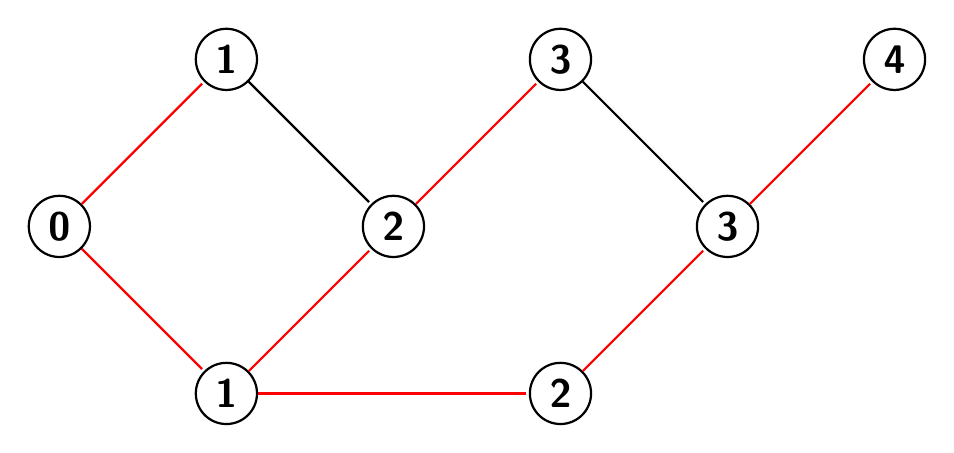
\begin{tikzpicture}[>=stealth',shorten >=1pt,auto,node distance=3cm,
    thick,main node/.style={circle,draw,font=\sffamily\Large\bfseries}]
    \node[main node] (1) {0};
    \node[main node] (2) [above right of=1] {1};
    \node[main node] (3) [below right of=1] {1};
    \node[main node] (4) [below right of=2] {2};
    \node[main node] (5) [above right of=4] {3};
    \node[main node] (6) [below right of=4] {2};
    \node[main node] (7) [above right of=6] {3};
    \node[main node] (8) [above right of=7] {4};
    \path[every node/.style={font=\sffamily\small}]
    (1) edge [draw=red] node [left] {} (2)
    edge [draw=red] node [left] {} (3)
    (2) edge node [left] {} (4) 
    (3) edge [draw=red] node [left] {} (4)
    (3) edge [draw=red] node [below left] {} (6)
    (4) edge [draw=red] node [left] {} (5)
    (5) edge node [left] {} (7)
    (6) edge [draw=red] node [left] {} (7)
    (7) edge [draw=red] node [left] {} (8);
    \end{tikzpicture}
\end{frame}

\begin{frame}{Breadth-First Search}{Results}
    \begin{columns}
        \column{.5\textwidth}
            Message Complexity: \\
            \hspace*{\parindent} $\mathcal{O}(n|E|)$ \\
            \pause
            \small
            \begin{itemize}
                \item A node, say $i_k$, can acquire up to $n$ estimates of its distance to $i_0$: $\to$ $O(n)$;
                \item In the worst case, these estimates are given to $i_k$ in a decreasing order, so each estimate causes an update which has to be propagated.
                \item In the worst case, each update is also propagated throughout all edges in the network: $\to$ $O(n|E|)$.
            \end{itemize}
        \pause
        \column{.5\textwidth}
            \normalsize
            Time Complexity:
            \hspace*{\parindent} $\mathcal{O}(diam \times n(l + d))$ \\
            \pause
            \small
            \begin{itemize}
                \item The length of a shortest path from $i_0$ to any node is at most $diam$. $\to$ $O(diam)$
                \item In the worst case, a maximum of $n$ messages are ever in any channel.
                \item In the worst case, all the processes take the maximum computation time, and all the channels take the maximum delivery time. $\to$ $O(diam \times n(l +d))$\\ 
            \end{itemize}           
    \end{columns} 
\end{frame}

\section{Bellman-Ford}
\begin{frame}{Bellman-Ford}{Algorithm}
    \normalsize
	The Bellman-Ford algorithm can be used to find a Minimum Spanning Tree. \\
    \vspace{12pt}
    \pause
    \textbf{Requirements}:
    \begin{enumerate}
        \item A \textbf{weighted}, undirected network graph;
        \item A start node $i_0$. 
    \end{enumerate}
    \pause
    \vspace{12pt}
    \textbf{Result}: \\
    A minimum spanning tree of the network graph.
\end{frame}

\begin{frame}{AsynchBFS}{Algorithm}
    \begin{block}{Transitions}
        \vspace{2mm}
        \begin{columns}
            \column{.5\textwidth}
            $\mathbf{send(m)_{i, j}:}$\\ 
            \emph{Precondition}: \\ 
            \small $m$ is first on $send(j)$ \\
            \normalsize \emph{Effect}: \\
            \small remove first element of $send(j)$
            \column{.5\textwidth}
            \normalsize $\mathbf{receive(m)_{i, j}: }$ \\
            \emph{Effect}: \\
            \small
            \begin{tcolorbox}[colframe=red]
                if $m+1 < dist$ then \\
                \hspace*{\parindent} $dist := m+1$ \\
                \hspace*{\parindent} $parent = j$ \\
                \hspace*{\parindent} for all $k \in nbrs - \{j\}$ do \\
                \hspace*{\parindent} \hspace*{\parindent} add $dist$ to $send(k)$ \\
            \end{tcolorbox}
        \end{columns}
    \end{block}
\end{frame}

\begin{frame}{Bellman-Ford}{Algorithm}
    \begin{block}{Transitions}
        \vspace{2mm}
        \begin{columns}
            \column{.5\textwidth}
            $\mathbf{send(m)_{i, j}:}$\\ 
            \emph{Precondition}: \\ 
            \small $m$ is first on $send(j)$ \\
            \normalsize \emph{Effect}: \\
            \small remove first element of $send(j)$
            \column{.5\textwidth}
            \normalsize $\mathbf{receive(m)_{i, j}: }$ \\
            \emph{Effect}: \\
            \small
            \begin{tcolorbox}[colframe=red]
                if $w + weight(j, i) < dist$ then \\
                \hspace*{\parindent} $dist := w + weight(j, i)$ \\
                \hspace*{\parindent} $parent = j$ \\
                \hspace*{\parindent} for all $k \in nbrs - \{j\}$ do \\
                \hspace*{\parindent} \hspace*{\parindent} add $dist$ to $send(k)$ \\
            \end{tcolorbox}
        \end{columns}
    \end{block}
\end{frame}

\begin{frame}{Bellman-Ford}{Complexity}
	\textbf{Message Complexity}: \\
    \vspace{8pt}
    \pause
	$\mathcal{O}(n^n |E|)$ \\
    \vspace{8pt}
    \pause
    \small
    The number of messages sent on each channel $C_{i, j}$ is proportional to the number of different distance estimates the process $i$ receives. \\
    \vspace{8pt}
    \pause
    In the worst case, each estimate is better than the preceding one and it has to be propagated to all neighbors. \\
    \vspace{8pt}
    \pause 
    The number of different estimates received is bounded on the number of distinct single paths from $i_0$ to $i$ in the network graph: $\mathcal{O}(n^n)$.
\end{frame}

\begin{frame}{Bellman-Ford}{Complexity}
    \textbf{Message Complexity}: \\
    \vspace{8pt}
    $\mathbb{O}(n^n |E|)$ \\
    \vspace{8pt}
    \small
    The number of messages sent on each channel $C_{i, j}$ is proportional to the number of different distance estimates the process $i$ receives. \\
    \vspace{8pt}
    In the worst case, each estimate is better than the preceding one and it has to be propagated to all neighbors. \\
    \vspace{8pt}
    \textbf{The number of different estimates received is bounded on the number of distinct single paths from $i_0$ to $i$ in the network graph}: $\mathbb{O}(n^n)$.
\end{frame}

\begin{frame}{Bellman-Ford}{Complexity (1 of 5)}
\begin{center}
\begin{columns}
    \begin{column}{.5\textwidth}
        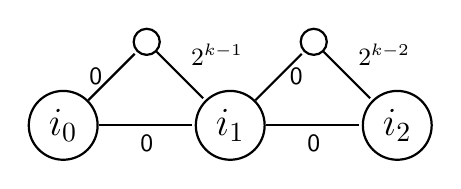
\begin{tikzpicture}[>=stealth',shorten >=1pt,auto,node distance=1.5cm,
        thick,main node/.style={circle,draw,font=\sffamily\Large\bfseries}]
        \node[main node] (0) {$i_0$};
        \node[main node] (1) [above right of=0] {};
        \node[main node] (2) [below right of=1] {$i_1$};
        \node[main node] (3) [above right of=2] {};
        \node[main node] (4) [below right of=3] {$i_2$};
        
        \path[every node/.style={font=\sffamily\small}]
        (0) edge node [left] {0} (1)
        (1) edge node [above right] {$2^{k-1}$} (2)
        (0) edge node [below] {0} (2) 
        (2) edge node [right] {0} (3)
        (3) edge node [above right] {$2^{k-2}$} (4)
        (2) edge node [below] {0} (4)
        ;
        \end{tikzpicture}
   \end{column}
   \begin{column}{.5\textwidth}
      \begin{tikzpicture}[>=stealth',shorten >=1pt,auto,node distance=1.5cm,
      thick,main node/.style={circle,draw,font=\sffamily\Large\bfseries}]
      \node[main node] (0) {$i_{k-1}$};
      \node[main node] (1) [above right of=0] {};
      \node[main node] (2) [below right of=1] {$i_k$};
      \node[main node] (4) [below right of=3] {$i_{k+1}$};
      \node[draw=none] (5) [above left of=0] {};
      
      \path[every node/.style={font=\sffamily\small}]
      (0) edge node [above left] {0} (1)
      (1) edge node [above right] {$2^0$} (2)
      (0) edge node [below] {0} (2) 
      (2) edge node [below] {0} (4)
      (0) edge node [above right] {$2^1$} (5)
      ;
      \end{tikzpicture} 
   \end{column}
\end{columns}
\end{center}
In graphs like this one, $i_k$ can actually receive $O(2^n)$ distance estimates. 
\end{frame}

\begin{frame}{Bellman-Ford}{Complexity (2 of 5)}
    \begin{center}
        \begin{columns}
            \begin{column}{.5\textwidth}
                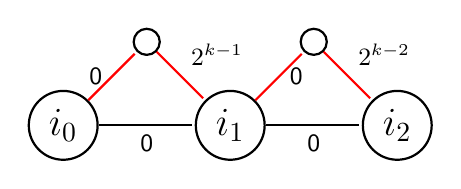
\begin{tikzpicture}[>=stealth',shorten >=1pt,auto,node distance=1.5cm,
                thick,main node/.style={circle,draw,font=\sffamily\Large\bfseries}]
                \node[main node] (0) {$i_0$};
                \node[main node] (1) [above right of=0] {};
                \node[main node] (2) [below right of=1] {$i_1$};
                \node[main node] (3) [above right of=2] {};
                \node[main node] (4) [below right of=3] {$i_2$};
                
                \path[every node/.style={font=\sffamily\small}]
                (0) edge[draw=red] node [left] {0} (1)
                (1) edge[draw=red] node [above right] {$2^{k-1}$} (2)
                (0) edge node [below] {0} (2) 
                (2) edge[draw=red] node [right] {0} (3)
                (3) edge[draw=red] node [above right] {$2^{k-2}$} (4)
                (2) edge node [below] {0} (4)
                ;
                \end{tikzpicture}
            \end{column}
            \begin{column}{.5\textwidth}
                \begin{tikzpicture}[>=stealth',shorten >=1pt,auto,node distance=1.5cm,
                thick,main node/.style={circle,draw,font=\sffamily\Large\bfseries}]
                \node[main node] (0) {$i_{k-1}$};
                \node[main node] (1) [above right of=0] {};
                \node[main node] (2) [below right of=1] {$i_k$};
                \node[main node] (4) [below right of=3] {$i_{k+1}$};
                \node[draw=none] (5) [above left of=0] {};
                \node[draw=none] (6) [left of=0] {};
                
                \path[every node/.style={font=\sffamily\small}]
                (0) edge[draw=red] node [above left] {0} (1)
                (1) edge[draw=red] node [above right] {$2^0$} (2)
                (0) edge node [below] {0} (2) 
                (2) edge node [below] {0} (4)
                (0) edge[draw=red] node [above right] {$2^1$} (5)
                (0) edge node {0} (6)
                ;
                \end{tikzpicture} 
            \end{column}
        \end{columns}
    \end{center}
    Current estimate: $2^k-1$
\end{frame}

\begin{frame}{Bellman-Ford}{Complexity (3 of 5)}
    \begin{center}
        \begin{columns}
            \begin{column}{.5\textwidth}
                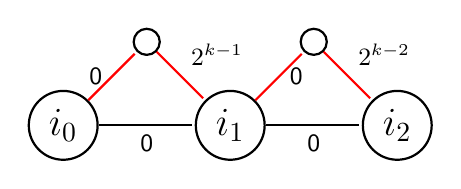
\begin{tikzpicture}[>=stealth',shorten >=1pt,auto,node distance=1.5cm,
                thick,main node/.style={circle,draw,font=\sffamily\Large\bfseries}]
                \node[main node] (0) {$i_0$};
                \node[main node] (1) [above right of=0] {};
                \node[main node] (2) [below right of=1] {$i_1$};
                \node[main node] (3) [above right of=2] {};
                \node[main node] (4) [below right of=3] {$i_2$};
                
                \path[every node/.style={font=\sffamily\small}]
                (0) edge[draw=red] node [left] {0} (1)
                (1) edge[draw=red] node [above right] {$2^{k-1}$} (2)
                (0) edge node [below] {0} (2) 
                (2) edge[draw=red] node [right] {0} (3)
                (3) edge[draw=red] node [above right] {$2^{k-2}$} (4)
                (2) edge node [below] {0} (4)
                ;
                \end{tikzpicture}
            \end{column}
            \begin{column}{.5\textwidth}
                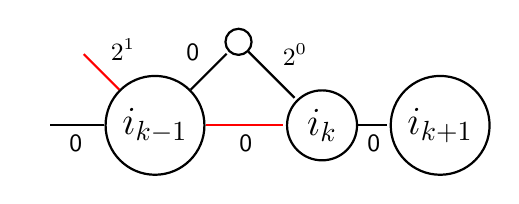
\begin{tikzpicture}[>=stealth',shorten >=1pt,auto,node distance=1.5cm,
                thick,main node/.style={circle,draw,font=\sffamily\Large\bfseries}]
                \node[main node] (0) {$i_{k-1}$};
                \node[main node] (1) [above right of=0] {};
                \node[main node] (2) [below right of=1] {$i_k$};
                \node[main node] (4) [right of=2] {$i_{k+1}$};
                \node[draw=none] (5) [above left of=0] {};
                \node[draw=none] (6) [left of=0] {};
                
                \path[every node/.style={font=\sffamily\small}]
                (0) edge node [above left] {0} (1)
                (1) edge node [above right] {$2^0$} (2)
                (0) edge[draw=red] node [below] {0} (2) 
                (2) edge node [below] {0} (4)
                (0) edge[draw=red] node [above right] {$2^1$} (5)
                (0) edge node {0} (6)
                ;
                \end{tikzpicture} 
            \end{column}
        \end{columns}
    \end{center}
    Current estimate: $2^k-2$
\end{frame}

\begin{frame}{Bellman-Ford}{Complexity (4 of 5)}
    \begin{center}
        \begin{columns}
            \begin{column}{.5\textwidth}
                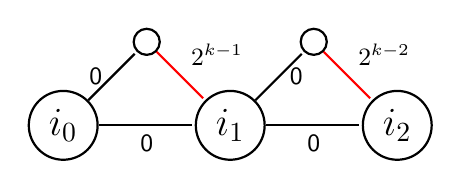
\begin{tikzpicture}[>=stealth',shorten >=1pt,auto,node distance=1.5cm,
                thick,main node/.style={circle,draw,font=\sffamily\Large\bfseries}]
                \node[main node] (0) {$i_0$};
                \node[main node] (1) [above right of=0] {};
                \node[main node] (2) [below right of=1] {$i_1$};
                \node[main node] (3) [above right of=2] {};
                \node[main node] (4) [below right of=3] {$i_2$};
                
                \path[every node/.style={font=\sffamily\small}]
                (0) edge node [left] {0} (1)
                (1) edge[draw=red] node [above right] {$2^{k-1}$} (2)
                (0) edge node [below] {0} (2) 
                (2) edge node [right] {0} (3)
                (3) edge[draw=red] node [above right] {$2^{k-2}$} (4)
                (2) edge node [below] {0} (4)
                ;
                \end{tikzpicture}
            \end{column}
            \begin{column}{.5\textwidth}
                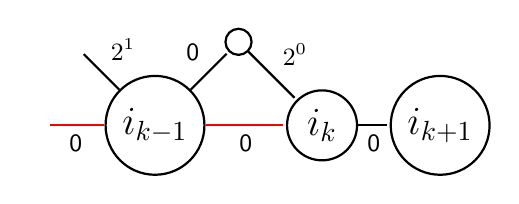
\begin{tikzpicture}[>=stealth',shorten >=1pt,auto,node distance=1.5cm,
                thick,main node/.style={circle,draw,font=\sffamily\Large\bfseries}]
                \node[main node] (0) {$i_{k-1}$};
                \node[main node] (1) [above right of=0] {};
                \node[main node] (2) [below right of=1] {$i_k$};
                \node[main node] (4) [right of=2] {$i_{k+1}$};
                \node[draw=none] (5) [above left of=0] {};
                \node[draw=none] (6) [left of=0] {};
                
                \path[every node/.style={font=\sffamily\small}]
                (0) edge node [above left] {0} (1)
                (1) edge node [above right] {$2^0$} (2)
                (0) edge[draw=red] node [below] {0} (2) 
                (2) edge node [below] {0} (4)
                (0) edge node [above right] {$2^1$} (5)
                (0) edge[draw=red] node {0} (6)
                ;
                \end{tikzpicture} 
            \end{column}
        \end{columns}
    \end{center}
    Current estimate: $2^k-4$.
\end{frame}

\begin{frame}{Bellman-Ford}{Complexity (5 of 5)}
    \begin{center}
        \begin{columns}
            \begin{column}{.5\textwidth}
                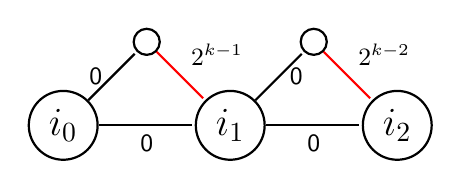
\begin{tikzpicture}[>=stealth',shorten >=1pt,auto,node distance=1.5cm,
                thick,main node/.style={circle,draw,font=\sffamily\Large\bfseries}]
                \node[main node] (0) {$i_0$};
                \node[main node] (1) [above right of=0] {};
                \node[main node] (2) [below right of=1] {$i_1$};
                \node[main node] (3) [above right of=2] {};
                \node[main node] (4) [below right of=3] {$i_2$};
                
                \path[every node/.style={font=\sffamily\small}]
                (0) edge node [left] {0} (1)
                (1) edge[draw=red] node [above right] {$2^{k-1}$} (2)
                (0) edge node [below] {0} (2) 
                (2) edge node [right] {0} (3)
                (3) edge[draw=red] node [above right] {$2^{k-2}$} (4)
                (2) edge node [below] {0} (4)
                ;
                \end{tikzpicture}
            \end{column}
            \begin{column}{.5\textwidth}
                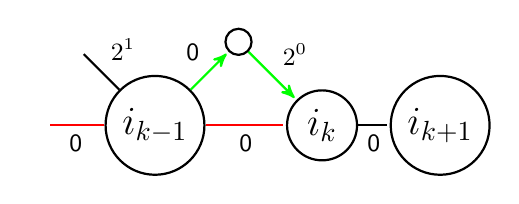
\begin{tikzpicture}[>=stealth',shorten >=1pt,auto,node distance=1.5cm,
                thick,main node/.style={circle,draw,font=\sffamily\Large\bfseries}]
                \node[main node] (0) {$i_{k-1}$};
                \node[main node] (1) [above right of=0] {};
                \node[main node] (2) [below right of=1] {$i_k$};
                \node[main node] (4) [right of=2] {$i_{k+1}$};
                \node[draw=none] (5) [above left of=0] {};
                \node[draw=none] (6) [left of=0] {};
                
                \path[every node/.style={font=\sffamily\small}]
                (0) edge[draw=green, ->] node [above left] {0} (1)
                (1) edge[draw=green, ->] node [above right] {$2^0$} (2)
                (0) edge[draw=red] node [below] {0} (2) 
                (2) edge node [below] {0} (4)
                (0) edge node [above right] {$2^1$} (5)
                (0) edge[draw=red] node {0} (6)
                ;
                \end{tikzpicture} 
            \end{column}
        \end{columns}
    \end{center}
    Current estimate: $2^k-4$. However, by propagation through $i_{k-1}$, $i_k$ will also receive the $2^k-3$ estimate, even if it ignores it.
\end{frame}

\begin{frame}{Bellman-Ford}{Complexity}
    \textbf{Message Complexity}: \\
    \vspace{8pt}
    $\mathbb{O}(n^n |E|)$ \\
    \vspace{8pt}
    \small
    The number of messages sent on each channel $C_{i, j}$ is proportional to the number of different distance estimates the process $i$ receives. \\
    \vspace{8pt}
    In the worst case, each estimate is better than the preceding one and it has to be propagated to all neighbors. \\
    \vspace{8pt}
    \textbf{The number of different estimates received is bounded on the number of distinct single paths from $i_0$ to $i$ in the network graph}: $\mathbb{O}(n^n)$.
\end{frame}

\begin{frame}{Bellman-Ford}{Complexity}
    \normalsize
    \textbf{Time Complexity}: \\
    \vspace{12pt}
    \pause
    $\mathcal{O}(n^{n+1}(l+d))$ \\
\end{frame}

\begin{frame}{Thank You!}
    \large
    Any questions?
\end{frame}

\end{document}
